\documentclass[twoside]{book}

% Packages required by doxygen
\usepackage{calc}
\usepackage{doxygen}
\usepackage{graphicx}
\usepackage[utf8]{inputenc}
\usepackage{makeidx}
\usepackage{multicol}
\usepackage{multirow}
\usepackage{textcomp}
\usepackage[table]{xcolor}

% Font selection
\usepackage[T1]{fontenc}
\usepackage{mathptmx}
\usepackage[scaled=.90]{helvet}
\usepackage{courier}
\usepackage{amssymb}
\usepackage{sectsty}
\renewcommand{\familydefault}{\sfdefault}
\allsectionsfont{%
  \fontseries{bc}\selectfont%
  \color{darkgray}%
}
\renewcommand{\DoxyLabelFont}{%
  \fontseries{bc}\selectfont%
  \color{darkgray}%
}

% Page & text layout
\usepackage{geometry}
\geometry{%
  a4paper,%
  top=2.5cm,%
  bottom=2.5cm,%
  left=2.5cm,%
  right=2.5cm%
}
\tolerance=750
\hfuzz=15pt
\hbadness=750
\setlength{\emergencystretch}{15pt}
\setlength{\parindent}{0cm}
\setlength{\parskip}{0.2cm}
\makeatletter
\renewcommand{\paragraph}{%
  \@startsection{paragraph}{4}{0ex}{-1.0ex}{1.0ex}{%
    \normalfont\normalsize\bfseries\SS@parafont%
  }%
}
\renewcommand{\subparagraph}{%
  \@startsection{subparagraph}{5}{0ex}{-1.0ex}{1.0ex}{%
    \normalfont\normalsize\bfseries\SS@subparafont%
  }%
}
\makeatother

% Headers & footers
\usepackage{fancyhdr}
\pagestyle{fancyplain}
\fancyhead[LE]{\fancyplain{}{\bfseries\thepage}}
\fancyhead[CE]{\fancyplain{}{}}
\fancyhead[RE]{\fancyplain{}{\bfseries\leftmark}}
\fancyhead[LO]{\fancyplain{}{\bfseries\rightmark}}
\fancyhead[CO]{\fancyplain{}{}}
\fancyhead[RO]{\fancyplain{}{\bfseries\thepage}}
\fancyfoot[LE]{\fancyplain{}{}}
\fancyfoot[CE]{\fancyplain{}{}}
\fancyfoot[RE]{\fancyplain{}{\bfseries\scriptsize Generated on Tue Sep 30 2014 18\-:15\-:22 for Connect\-Four by Doxygen }}
\fancyfoot[LO]{\fancyplain{}{\bfseries\scriptsize Generated on Tue Sep 30 2014 18\-:15\-:22 for Connect\-Four by Doxygen }}
\fancyfoot[CO]{\fancyplain{}{}}
\fancyfoot[RO]{\fancyplain{}{}}
\renewcommand{\footrulewidth}{0.4pt}
\renewcommand{\chaptermark}[1]{%
  \markboth{#1}{}%
}
\renewcommand{\sectionmark}[1]{%
  \markright{\thesection\ #1}%
}

% Indices & bibliography
\usepackage{natbib}
\usepackage[titles]{tocloft}
\setcounter{tocdepth}{3}
\setcounter{secnumdepth}{5}
\makeindex

% Hyperlinks (required, but should be loaded last)
\usepackage{ifpdf}
\ifpdf
  \usepackage[pdftex,pagebackref=true]{hyperref}
\else
  \usepackage[ps2pdf,pagebackref=true]{hyperref}
\fi
\hypersetup{%
  colorlinks=true,%
  linkcolor=blue,%
  citecolor=blue,%
  unicode%
}

% Custom commands
\newcommand{\clearemptydoublepage}{%
  \newpage{\pagestyle{empty}\cleardoublepage}%
}


%===== C O N T E N T S =====

\begin{document}

% Titlepage & ToC
\hypersetup{pageanchor=false}
\pagenumbering{roman}
\begin{titlepage}
\vspace*{7cm}
\begin{center}%
{\Large Connect\-Four }\\
\vspace*{1cm}
{\large Generated by Doxygen 1.8.6}\\
\vspace*{0.5cm}
{\small Tue Sep 30 2014 18:15:22}\\
\end{center}
\end{titlepage}
\clearemptydoublepage
\tableofcontents
\clearemptydoublepage
\pagenumbering{arabic}
\hypersetup{pageanchor=true}

%--- Begin generated contents ---
\chapter{Hierarchical Index}
\section{\-Class \-Hierarchy}
\-This inheritance list is sorted roughly, but not completely, alphabetically\-:\begin{DoxyCompactList}
\item \contentsline{section}{\-Animation}{\pageref{structAnimation}}{}
\item \contentsline{section}{\-Board\-Column}{\pageref{classBoardColumn}}{}
\item \contentsline{section}{\-Connect\-Four\-Object}{\pageref{classConnectFourObject}}{}
\begin{DoxyCompactList}
\item \contentsline{section}{\-Connect\-Four\-Render\-Object}{\pageref{classConnectFourRenderObject}}{}
\begin{DoxyCompactList}
\item \contentsline{section}{\-Game\-Board\-Renderer}{\pageref{classGameBoardRenderer}}{}
\item \contentsline{section}{\-Game\-Coin\-Renderer}{\pageref{classGameCoinRenderer}}{}
\end{DoxyCompactList}
\item \contentsline{section}{\-Game\-Board}{\pageref{classGameBoard}}{}
\end{DoxyCompactList}
\item \contentsline{section}{\-Game}{\pageref{structGame}}{}
\item \contentsline{section}{\-Game\-Database}{\pageref{classGameDatabase}}{}
\item \contentsline{section}{\-Game\-Manager}{\pageref{classGameManager}}{}
\begin{DoxyCompactList}
\item \contentsline{section}{\-A\-I\-Game\-Manager}{\pageref{classAIGameManager}}{}
\item \contentsline{section}{\-T\-C\-P\-Game\-Manager}{\pageref{classTCPGameManager}}{}
\end{DoxyCompactList}
\item \contentsline{section}{\-Game\-Over\-Screen}{\pageref{classGameOverScreen}}{}
\item \contentsline{section}{\-Game\-Renderer}{\pageref{classGameRenderer}}{}
\item \contentsline{section}{\-Game\-Results}{\pageref{classGameResults}}{}
\item \contentsline{section}{\-Helper}{\pageref{classHelper}}{}
\item \contentsline{section}{\-Main\-Window}{\pageref{classMainWindow}}{}
\item \contentsline{section}{\-Min\-Max}{\pageref{classMinMax}}{}
\item \contentsline{section}{\-Network\-Adapter}{\pageref{classNetworkAdapter}}{}
\begin{DoxyCompactList}
\item \contentsline{section}{\-Game\-Client}{\pageref{classGameClient}}{}
\item \contentsline{section}{\-Game\-Server}{\pageref{classGameServer}}{}
\end{DoxyCompactList}
\item \contentsline{section}{\-Player}{\pageref{classPlayer}}{}
\item \contentsline{section}{\-Render\-Object}{\pageref{classRenderObject}}{}
\begin{DoxyCompactList}
\item \contentsline{section}{\-Connect\-Four\-Render\-Object}{\pageref{classConnectFourRenderObject}}{}
\end{DoxyCompactList}
\item \contentsline{section}{\-Settings}{\pageref{structSettings}}{}
\item \contentsline{section}{\-Settings\-Widget}{\pageref{classSettingsWidget}}{}
\end{DoxyCompactList}

\chapter{Class Index}
\section{\-Class \-List}
\-Here are the classes, structs, unions and interfaces with brief descriptions\-:\begin{DoxyCompactList}
\item\contentsline{section}{\hyperlink{classAIGameManager}{\-A\-I\-Game\-Manager} \\*\-Ai specific gamemanager }{\pageref{classAIGameManager}}{}
\item\contentsline{section}{\hyperlink{structAnimation}{\-Animation} \\*\-Handles animation state }{\pageref{structAnimation}}{}
\item\contentsline{section}{\hyperlink{classBoardColumn}{\-Board\-Column} \\*\-Column for the game board }{\pageref{classBoardColumn}}{}
\item\contentsline{section}{\hyperlink{classConnectFourObject}{\-Connect\-Four\-Object} \\*\-Base class for every connect four related class }{\pageref{classConnectFourObject}}{}
\item\contentsline{section}{\hyperlink{classConnectFourRenderObject}{\-Connect\-Four\-Render\-Object} \\*\-Base class for each renderable connect four object }{\pageref{classConnectFourRenderObject}}{}
\item\contentsline{section}{\hyperlink{structGame}{\-Game} \\*\-Data holder for game results }{\pageref{structGame}}{}
\item\contentsline{section}{\hyperlink{classGameBoard}{\-Game\-Board} \\*\hyperlink{structGame}{\-Game} board class representing game board }{\pageref{classGameBoard}}{}
\item\contentsline{section}{\hyperlink{classGameBoardRenderer}{\-Game\-Board\-Renderer} \\*\-Class that is responsible for rendering the gameboard }{\pageref{classGameBoardRenderer}}{}
\item\contentsline{section}{\hyperlink{classGameClient}{\-Game\-Client} \\*\-Class that is responsible for opening a tcp socket connection to the host }{\pageref{classGameClient}}{}
\item\contentsline{section}{\hyperlink{classGameCoinRenderer}{\-Game\-Coin\-Renderer} \\*\-Class that is responsible for rendering the coins added to the board }{\pageref{classGameCoinRenderer}}{}
\item\contentsline{section}{\hyperlink{classGameDatabase}{\-Game\-Database} \\*\-Singleton class that manages the game result database }{\pageref{classGameDatabase}}{}
\item\contentsline{section}{\hyperlink{classGameManager}{\-Game\-Manager} \\*\-Class that handles game states and instanciates renderer and board }{\pageref{classGameManager}}{}
\item\contentsline{section}{\hyperlink{classGameOverScreen}{\-Game\-Over\-Screen} \\*\-Class that handles game over screen }{\pageref{classGameOverScreen}}{}
\item\contentsline{section}{\hyperlink{classGameRenderer}{\-Game\-Renderer} \\*\-Handles \-Open\-G\-L window inside main window; }{\pageref{classGameRenderer}}{}
\item\contentsline{section}{\hyperlink{classGameResults}{\-Game\-Results} \\*\-Show previous games }{\pageref{classGameResults}}{}
\item\contentsline{section}{\hyperlink{classGameServer}{\-Game\-Server} \\*\-Class that handles server client connection }{\pageref{classGameServer}}{}
\item\contentsline{section}{\hyperlink{classHelper}{\-Helper} \\*\hyperlink{classHelper}{\-Helper} class for \-Connect \-Four }{\pageref{classHelper}}{}
\item\contentsline{section}{\hyperlink{classMainWindow}{\-Main\-Window} \\*\-Main window class }{\pageref{classMainWindow}}{}
\item\contentsline{section}{\hyperlink{classMinMax}{\-Min\-Max} \\*\-Negamax algorithm }{\pageref{classMinMax}}{}
\item\contentsline{section}{\hyperlink{classNetworkAdapter}{\-Network\-Adapter} \\*\-Base class for a network connection (server and client) }{\pageref{classNetworkAdapter}}{}
\item\contentsline{section}{\hyperlink{classPlayer}{\-Player} \\*\hyperlink{classPlayer}{\-Player} data holder }{\pageref{classPlayer}}{}
\item\contentsline{section}{\hyperlink{classRenderObject}{\-Render\-Object} \\*\-Abstract class for each renderable object }{\pageref{classRenderObject}}{}
\item\contentsline{section}{\hyperlink{structSettings}{\-Settings} \\*\-Data holder between ui and game }{\pageref{structSettings}}{}
\item\contentsline{section}{\hyperlink{classSettingsWidget}{\-Settings\-Widget} \\*\-Widget for settings }{\pageref{classSettingsWidget}}{}
\item\contentsline{section}{\hyperlink{classTCPGameManager}{\-T\-C\-P\-Game\-Manager} \\*\-Gamemanager that handles \-Network game related tasks }{\pageref{classTCPGameManager}}{}
\end{DoxyCompactList}

\chapter{Class Documentation}
\hypertarget{class_a_i_game_manager}{\section{A\-I\-Game\-Manager Class Reference}
\label{class_a_i_game_manager}\index{A\-I\-Game\-Manager@{A\-I\-Game\-Manager}}
}


ai specific gamemanager  




{\ttfamily \#include $<$aigamemanager.\-h$>$}

Inheritance diagram for A\-I\-Game\-Manager\-:\begin{figure}[H]
\begin{center}
\leavevmode
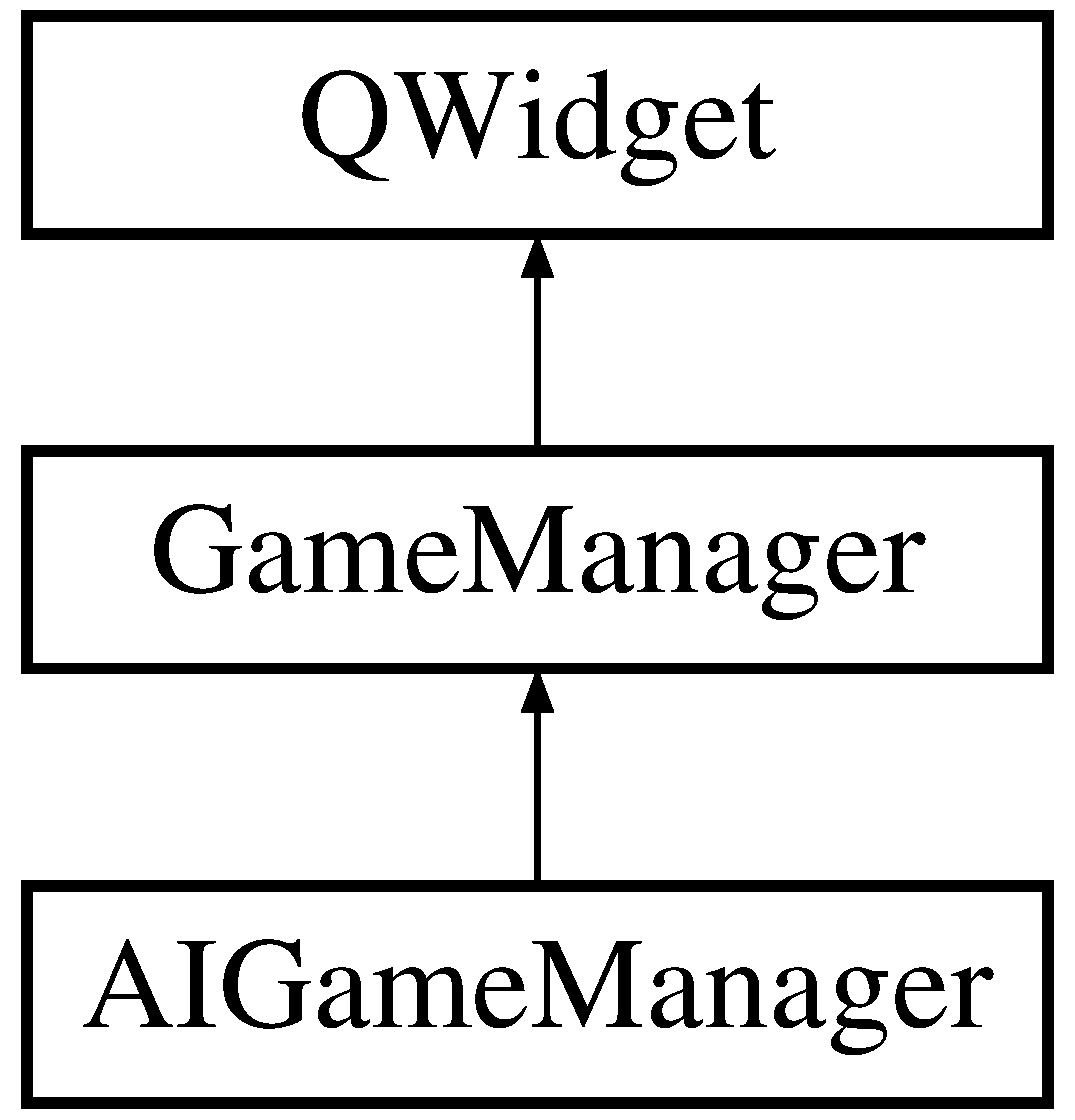
\includegraphics[height=3.000000cm]{class_a_i_game_manager}
\end{center}
\end{figure}
\subsection*{Public Slots}
\begin{DoxyCompactItemize}
\item 
\hypertarget{class_a_i_game_manager_a1dd46d003522dfad3572c0de445d1d20}{void {\bfseries mouse\-Press\-Event} (Q\-Mouse\-Event $\ast$event)}\label{class_a_i_game_manager_a1dd46d003522dfad3572c0de445d1d20}

\end{DoxyCompactItemize}
\subsection*{Public Member Functions}
\begin{DoxyCompactItemize}
\item 
\hypertarget{class_a_i_game_manager_a488945627859aff9401f1280f123bdc4}{{\bfseries A\-I\-Game\-Manager} (Q\-Widget $\ast$parent=0)}\label{class_a_i_game_manager_a488945627859aff9401f1280f123bdc4}

\item 
\hypertarget{class_a_i_game_manager_a00ceeb80c83e9b7951442ce695b9730f}{virtual void \hyperlink{class_a_i_game_manager_a00ceeb80c83e9b7951442ce695b9730f}{start\-Game} (\hyperlink{struct_settings}{Settings} settings)}\label{class_a_i_game_manager_a00ceeb80c83e9b7951442ce695b9730f}

\begin{DoxyCompactList}\small\item\em instanciates renderer and gameboard \end{DoxyCompactList}\item 
\hypertarget{class_a_i_game_manager_a91068d6c5076821cd5361efdbbc68fef}{virtual void \hyperlink{class_a_i_game_manager_a91068d6c5076821cd5361efdbbc68fef}{set\-Starting\-Player} (\hyperlink{struct_settings}{Settings} settings)}\label{class_a_i_game_manager_a91068d6c5076821cd5361efdbbc68fef}

\begin{DoxyCompactList}\small\item\em Sets the starting player depending wether ai should start. \end{DoxyCompactList}\end{DoxyCompactItemize}
\subsection*{Additional Inherited Members}


\subsection{Detailed Description}
ai specific gamemanager 

A\-I specific gamemanger that handles the ai players turn 

Definition at line 10 of file aigamemanager.\-h.



The documentation for this class was generated from the following files\-:\begin{DoxyCompactItemize}
\item 
aigamemanager.\-h\item 
aigamemanager.\-cpp\end{DoxyCompactItemize}

\hypertarget{struct_animation}{\section{Animation Struct Reference}
\label{struct_animation}\index{Animation@{Animation}}
}


Struct that handles animation state.  




{\ttfamily \#include $<$animation.\-h$>$}

\subsection*{Public Attributes}
\begin{DoxyCompactItemize}
\item 
\hypertarget{struct_animation_a82d1d99dc58d52abf27385cd556aa534}{bool {\bfseries bounce\-Up}}\label{struct_animation_a82d1d99dc58d52abf27385cd556aa534}

\item 
\hypertarget{struct_animation_aea31cea7c443a26db5be51260678c93f}{bool {\bfseries did\-Bounce}}\label{struct_animation_aea31cea7c443a26db5be51260678c93f}

\item 
\hypertarget{struct_animation_ab7b2041b8fe676c3980eb27feb3c24d7}{bool {\bfseries active}}\label{struct_animation_ab7b2041b8fe676c3980eb27feb3c24d7}

\item 
\hypertarget{struct_animation_a0e5e8258f63ad3af3889c05dadbd50dd}{int {\bfseries current\-Y}}\label{struct_animation_a0e5e8258f63ad3af3889c05dadbd50dd}

\item 
\hypertarget{struct_animation_a270b071f76360d3a3d354fdc82034273}{int {\bfseries end\-Y}}\label{struct_animation_a270b071f76360d3a3d354fdc82034273}

\item 
\hypertarget{struct_animation_a4a79cc62a84e6f59fe7a9671c45e9afa}{int {\bfseries position\-X}}\label{struct_animation_a4a79cc62a84e6f59fe7a9671c45e9afa}

\item 
\hypertarget{struct_animation_ab9869e44134973b0d48506e8948cce40}{int {\bfseries start\-Y}}\label{struct_animation_ab9869e44134973b0d48506e8948cce40}

\item 
\hypertarget{struct_animation_a5e1834181ba3fc0fb0c201c0f6060fd8}{int {\bfseries current\-Bounce\-Distance}}\label{struct_animation_a5e1834181ba3fc0fb0c201c0f6060fd8}

\item 
\hypertarget{struct_animation_a881ac177b0e6feeb173f2ab6c1ae2667}{int {\bfseries max\-Bounce\-Distance}}\label{struct_animation_a881ac177b0e6feeb173f2ab6c1ae2667}

\item 
\hypertarget{struct_animation_ad8d4d4bba5b9accfba17cc9ecf5f3b50}{float {\bfseries time}}\label{struct_animation_ad8d4d4bba5b9accfba17cc9ecf5f3b50}

\item 
\hypertarget{struct_animation_a4d5850dde030ebc98d8f7a4427390ee4}{Coin {\bfseries player}}\label{struct_animation_a4d5850dde030ebc98d8f7a4427390ee4}

\end{DoxyCompactItemize}


\subsection{Detailed Description}
Struct that handles animation state. 

Definition at line 10 of file animation.\-h.



The documentation for this struct was generated from the following file\-:\begin{DoxyCompactItemize}
\item 
animation.\-h\end{DoxyCompactItemize}

\hypertarget{class_board_column}{\section{Board\-Column Class Reference}
\label{class_board_column}\index{Board\-Column@{Board\-Column}}
}


column for the game board  




{\ttfamily \#include $<$boardcolumn.\-h$>$}

\subsection*{Public Member Functions}
\begin{DoxyCompactItemize}
\item 
\hypertarget{class_board_column_a8f088cd71325ffbdc839c101ca6a4fda}{{\bfseries Board\-Column} (int rows)}\label{class_board_column_a8f088cd71325ffbdc839c101ca6a4fda}

\item 
\hypertarget{class_board_column_adb1521008180835bd37572a1cda02ef8}{bool {\bfseries is\-Full} ()}\label{class_board_column_adb1521008180835bd37572a1cda02ef8}

\item 
\hypertarget{class_board_column_a09589c8bd6912dab8a7fb27500002553}{int {\bfseries get\-Current\-Amount\-Of\-Coins} ()}\label{class_board_column_a09589c8bd6912dab8a7fb27500002553}

\item 
\hypertarget{class_board_column_a060fd86473c5df6a98449e317bc2a364}{bool \hyperlink{class_board_column_a060fd86473c5df6a98449e317bc2a364}{add\-Coin} (Coin coin)}\label{class_board_column_a060fd86473c5df6a98449e317bc2a364}

\begin{DoxyCompactList}\small\item\em adds an coin to the boardcolumn \end{DoxyCompactList}\item 
Coin \hyperlink{class_board_column_a8b8107a2cb462ffd73d484b6e1d9b359}{get\-Coin} (int index)
\begin{DoxyCompactList}\small\item\em returns the coin at the specific index \end{DoxyCompactList}\item 
\hypertarget{class_board_column_ad4b43af3abf8de3332378529b7d5e743}{void \hyperlink{class_board_column_ad4b43af3abf8de3332378529b7d5e743}{remove\-Last\-Coin} ()}\label{class_board_column_ad4b43af3abf8de3332378529b7d5e743}

\begin{DoxyCompactList}\small\item\em removes the last added coin \end{DoxyCompactList}\item 
\hypertarget{class_board_column_a316e15e6e992dc3e0bba17289bad228a}{void \hyperlink{class_board_column_a316e15e6e992dc3e0bba17289bad228a}{clear} ()}\label{class_board_column_a316e15e6e992dc3e0bba17289bad228a}

\begin{DoxyCompactList}\small\item\em clears the boardcolumn \end{DoxyCompactList}\item 
\hypertarget{class_board_column_a8f088cd71325ffbdc839c101ca6a4fda}{{\bfseries Board\-Column} (int rows)}\label{class_board_column_a8f088cd71325ffbdc839c101ca6a4fda}

\item 
\hypertarget{class_board_column_adb1521008180835bd37572a1cda02ef8}{bool {\bfseries is\-Full} ()}\label{class_board_column_adb1521008180835bd37572a1cda02ef8}

\item 
\hypertarget{class_board_column_a09589c8bd6912dab8a7fb27500002553}{int {\bfseries get\-Current\-Amount\-Of\-Coins} ()}\label{class_board_column_a09589c8bd6912dab8a7fb27500002553}

\item 
\hypertarget{class_board_column_a060fd86473c5df6a98449e317bc2a364}{bool {\bfseries add\-Coin} (Coin coin)}\label{class_board_column_a060fd86473c5df6a98449e317bc2a364}

\item 
\hypertarget{class_board_column_a8b8107a2cb462ffd73d484b6e1d9b359}{Coin {\bfseries get\-Coin} (int index)}\label{class_board_column_a8b8107a2cb462ffd73d484b6e1d9b359}

\end{DoxyCompactItemize}


\subsection{Detailed Description}
column for the game board 

Definition at line 8 of file boardcolumn.\-h.



\subsection{Member Function Documentation}
\hypertarget{class_board_column_a8b8107a2cb462ffd73d484b6e1d9b359}{\index{Board\-Column@{Board\-Column}!get\-Coin@{get\-Coin}}
\index{get\-Coin@{get\-Coin}!BoardColumn@{Board\-Column}}
\subsubsection[{get\-Coin}]{\setlength{\rightskip}{0pt plus 5cm}Coin Board\-Column\-::get\-Coin (
\begin{DoxyParamCaption}
\item[{int}]{index}
\end{DoxyParamCaption}
)\hspace{0.3cm}{\ttfamily [inline]}}}\label{class_board_column_a8b8107a2cb462ffd73d484b6e1d9b359}


returns the coin at the specific index 


\begin{DoxyParams}{Parameters}
{\em index} & the index of the coin \\
\hline
\end{DoxyParams}


Definition at line 46 of file boardcolumn.\-h.



The documentation for this class was generated from the following files\-:\begin{DoxyCompactItemize}
\item 
boardcolumn.\-h\item 
column.\-h\item 
column.\-cpp\end{DoxyCompactItemize}

\hypertarget{class_chat_widget}{\section{Chat\-Widget Class Reference}
\label{class_chat_widget}\index{Chat\-Widget@{Chat\-Widget}}
}
Inheritance diagram for Chat\-Widget\-:\begin{figure}[H]
\begin{center}
\leavevmode
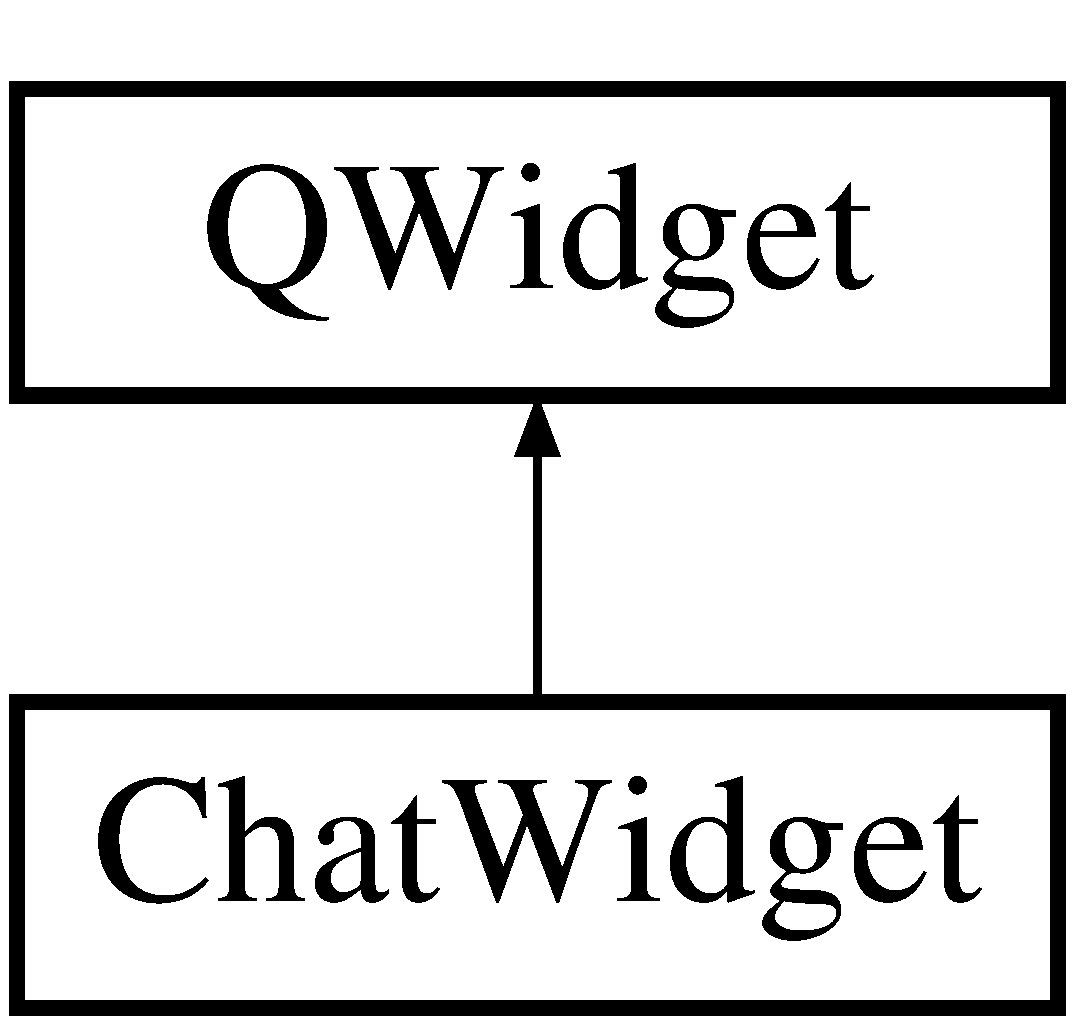
\includegraphics[height=2.000000cm]{class_chat_widget}
\end{center}
\end{figure}
\subsection*{Public Member Functions}
\begin{DoxyCompactItemize}
\item 
\hypertarget{class_chat_widget_a605bb01b4520874d34e3882edb70be38}{{\bfseries Chat\-Widget} (Q\-Widget $\ast$parent=0)}\label{class_chat_widget_a605bb01b4520874d34e3882edb70be38}

\item 
\hypertarget{class_chat_widget_a0919f7952cb4525f7966411a2c36da8f}{void {\bfseries init} (\hyperlink{class_t_c_p_game_manager}{T\-C\-P\-Game\-Manager} $\ast$tcp\-Game\-Manager)}\label{class_chat_widget_a0919f7952cb4525f7966411a2c36da8f}

\end{DoxyCompactItemize}


\subsection{Detailed Description}


Definition at line 10 of file chatwidget.\-h.



The documentation for this class was generated from the following files\-:\begin{DoxyCompactItemize}
\item 
chatwidget.\-h\item 
chatwidget.\-cpp\end{DoxyCompactItemize}

\hypertarget{class_connect_four_object}{\section{Connect\-Four\-Object Class Reference}
\label{class_connect_four_object}\index{Connect\-Four\-Object@{Connect\-Four\-Object}}
}


base class for every connect four related class  




{\ttfamily \#include $<$connectfourobject.\-h$>$}

Inheritance diagram for Connect\-Four\-Object\-:\begin{figure}[H]
\begin{center}
\leavevmode
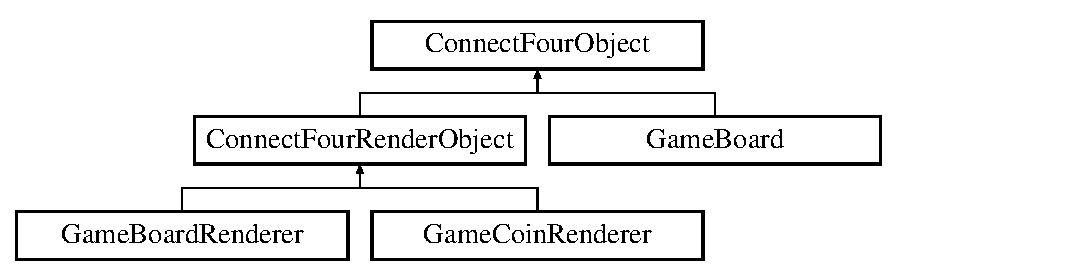
\includegraphics[height=3.000000cm]{class_connect_four_object}
\end{center}
\end{figure}
\subsection*{Public Member Functions}
\begin{DoxyCompactItemize}
\item 
\hypertarget{class_connect_four_object_a6dabab64cdbd0b264aebf42435dd901b}{{\bfseries Connect\-Four\-Object} (int width, int height)}\label{class_connect_four_object_a6dabab64cdbd0b264aebf42435dd901b}

\end{DoxyCompactItemize}
\subsection*{Protected Attributes}
\begin{DoxyCompactItemize}
\item 
\hypertarget{class_connect_four_object_ae6e240f90182a3ff58790a1307ccd1b1}{int {\bfseries m\-\_\-\-Rows}}\label{class_connect_four_object_ae6e240f90182a3ff58790a1307ccd1b1}

\item 
\hypertarget{class_connect_four_object_a6a2622a917669b269f88af84f25425eb}{int {\bfseries m\-\_\-\-Columns}}\label{class_connect_four_object_a6a2622a917669b269f88af84f25425eb}

\end{DoxyCompactItemize}


\subsection{Detailed Description}
base class for every connect four related class 

Definition at line 5 of file connectfourobject.\-h.



The documentation for this class was generated from the following file\-:\begin{DoxyCompactItemize}
\item 
connectfourobject.\-h\end{DoxyCompactItemize}

\hypertarget{class_connect_four_render_object}{\section{Connect\-Four\-Render\-Object Class Reference}
\label{class_connect_four_render_object}\index{Connect\-Four\-Render\-Object@{Connect\-Four\-Render\-Object}}
}


base class for each renderable connect four object  




{\ttfamily \#include $<$connectfourrenderobject.\-h$>$}

Inheritance diagram for Connect\-Four\-Render\-Object\-:\begin{figure}[H]
\begin{center}
\leavevmode
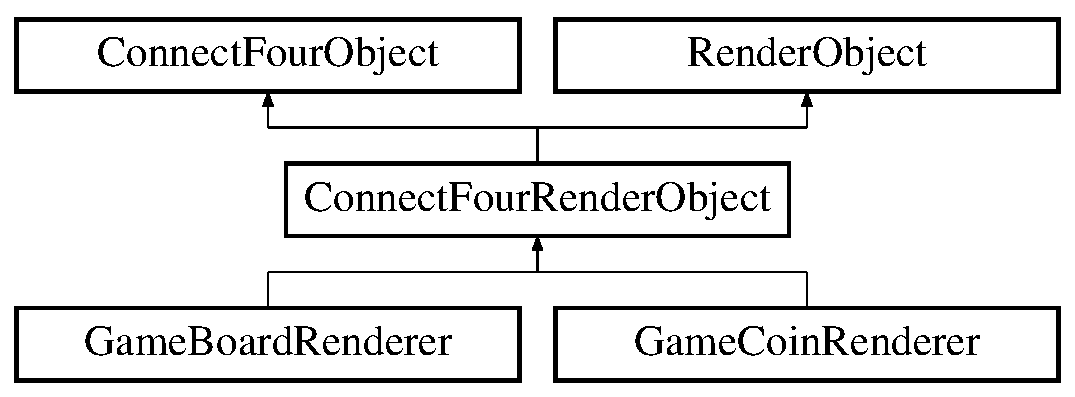
\includegraphics[height=3.000000cm]{class_connect_four_render_object}
\end{center}
\end{figure}
\subsection*{Public Member Functions}
\begin{DoxyCompactItemize}
\item 
\hypertarget{class_connect_four_render_object_a8f005868218af313f4d4cbde8041a10f}{{\bfseries Connect\-Four\-Render\-Object} (int width, int height, float cell\-Size, Design design)}\label{class_connect_four_render_object_a8f005868218af313f4d4cbde8041a10f}

\item 
\hypertarget{class_connect_four_render_object_a9b29bbc57d9985db1075a1b147b15801}{virtual void {\bfseries resize} (int width, int height)}\label{class_connect_four_render_object_a9b29bbc57d9985db1075a1b147b15801}

\end{DoxyCompactItemize}
\subsection*{Protected Member Functions}
\begin{DoxyCompactItemize}
\item 
\hypertarget{class_connect_four_render_object_a4b8e9a3cc37ba5b6a6baf341f18f8328}{void {\bfseries draw\-Primitive} ()}\label{class_connect_four_render_object_a4b8e9a3cc37ba5b6a6baf341f18f8328}

\item 
\hypertarget{class_connect_four_render_object_a04ad47593cfd44bdda2ae4ba833f5a18}{float {\bfseries get\-Coin\-Radius} ()}\label{class_connect_four_render_object_a04ad47593cfd44bdda2ae4ba833f5a18}

\end{DoxyCompactItemize}
\subsection*{Protected Attributes}
\begin{DoxyCompactItemize}
\item 
\hypertarget{class_connect_four_render_object_a507319d76cc95bd30ca5a8e4e5e4e5c6}{float {\bfseries m\-\_\-\-Cell\-Size}}\label{class_connect_four_render_object_a507319d76cc95bd30ca5a8e4e5e4e5c6}

\item 
\hypertarget{class_connect_four_render_object_a039a66092b64a1b5940118d7430ba302}{Design {\bfseries m\-\_\-\-Design}}\label{class_connect_four_render_object_a039a66092b64a1b5940118d7430ba302}

\item 
\hypertarget{class_connect_four_render_object_aa864124c16d148218a340af0340d6ddf}{float {\bfseries m\-\_\-\-Scale}}\label{class_connect_four_render_object_aa864124c16d148218a340af0340d6ddf}

\end{DoxyCompactItemize}


\subsection{Detailed Description}
base class for each renderable connect four object 

Definition at line 11 of file connectfourrenderobject.\-h.



The documentation for this class was generated from the following file\-:\begin{DoxyCompactItemize}
\item 
connectfourrenderobject.\-h\end{DoxyCompactItemize}

\hypertarget{struct_game}{\section{Game Struct Reference}
\label{struct_game}\index{Game@{Game}}
}


data holder for game results  




{\ttfamily \#include $<$game.\-h$>$}

\subsection*{Public Member Functions}
\begin{DoxyCompactItemize}
\item 
\hypertarget{struct_game_a044fef9d8dfbbece3bafa8762991d50a}{{\bfseries Game} (Result result)}\label{struct_game_a044fef9d8dfbbece3bafa8762991d50a}

\item 
\hypertarget{struct_game_a43e6e19cc502235683d5014c78f37bbd}{{\bfseries Game} (Result result, \hyperlink{class_player}{Player} winner, \hyperlink{class_player}{Player} loser, double duration=0.\-0)}\label{struct_game_a43e6e19cc502235683d5014c78f37bbd}

\item 
\hypertarget{struct_game_a0aa609437b4295dba61e18b7e01cc2a7}{Q\-String {\bfseries to\-String} ()}\label{struct_game_a0aa609437b4295dba61e18b7e01cc2a7}

\end{DoxyCompactItemize}
\subsection*{Public Attributes}
\begin{DoxyCompactItemize}
\item 
\hypertarget{struct_game_a9649ed9f4a7e37744396a793d345a222}{Result {\bfseries result}}\label{struct_game_a9649ed9f4a7e37744396a793d345a222}

\item 
\hypertarget{struct_game_a590df81200f797fd5bef8c5968a2ea1b}{\hyperlink{class_player}{Player} {\bfseries winner}}\label{struct_game_a590df81200f797fd5bef8c5968a2ea1b}

\item 
\hypertarget{struct_game_a151b35fd4e46d2152eb7e5d196e0b4de}{\hyperlink{class_player}{Player} {\bfseries loser}}\label{struct_game_a151b35fd4e46d2152eb7e5d196e0b4de}

\item 
\hypertarget{struct_game_a5ec0d2343999d0f1f2f1ec20a24c343b}{double {\bfseries duration}}\label{struct_game_a5ec0d2343999d0f1f2f1ec20a24c343b}

\end{DoxyCompactItemize}


\subsection{Detailed Description}
data holder for game results 

Definition at line 18 of file game.\-h.



The documentation for this struct was generated from the following file\-:\begin{DoxyCompactItemize}
\item 
game.\-h\end{DoxyCompactItemize}

\hypertarget{class_game_audio_manager}{\section{Game\-Audio\-Manager Class Reference}
\label{class_game_audio_manager}\index{Game\-Audio\-Manager@{Game\-Audio\-Manager}}
}


Singleton Class that handles audio loading and playback.  




{\ttfamily \#include $<$gameaudiomanager.\-h$>$}

Inheritance diagram for Game\-Audio\-Manager\-:\begin{figure}[H]
\begin{center}
\leavevmode
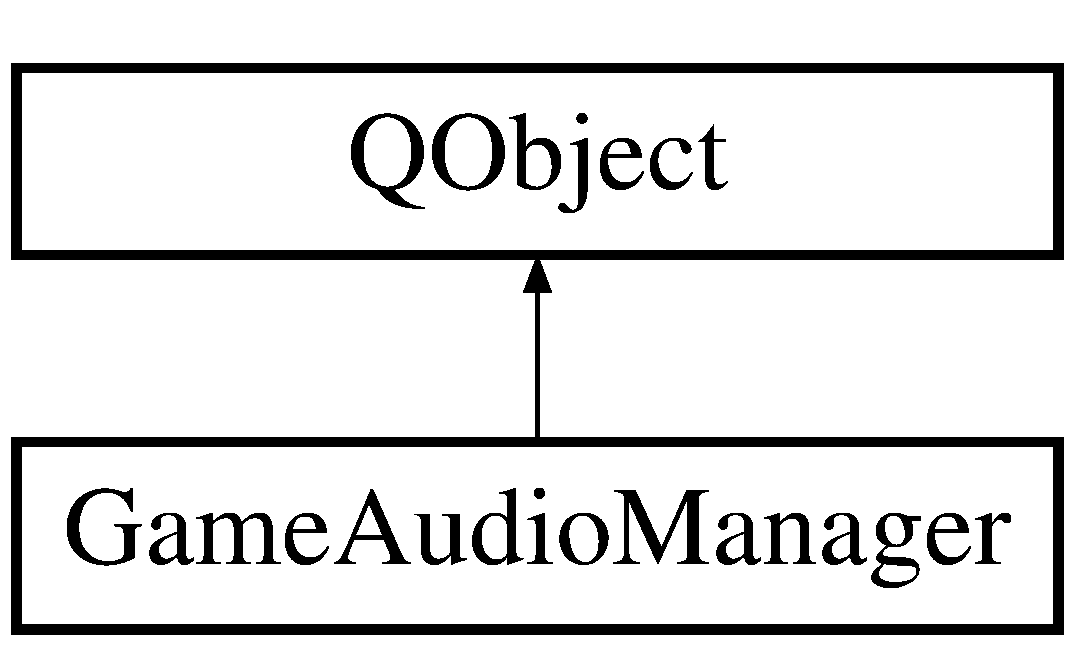
\includegraphics[height=2.000000cm]{class_game_audio_manager}
\end{center}
\end{figure}
\subsection*{Public Member Functions}
\begin{DoxyCompactItemize}
\item 
void \hyperlink{class_game_audio_manager_ace62a41952c9c84d96ff604bb1170c44}{add\-Audio} (Q\-String name, std\-::shared\-\_\-ptr$<$ Q\-Sound $>$ sound)
\begin{DoxyCompactList}\small\item\em adds audio \end{DoxyCompactList}\item 
\hypertarget{class_game_audio_manager_a92a40349d9d48bdd0f9f8599db854cba}{void \hyperlink{class_game_audio_manager_a92a40349d9d48bdd0f9f8599db854cba}{play\-Audio} (Q\-String name)}\label{class_game_audio_manager_a92a40349d9d48bdd0f9f8599db854cba}

\begin{DoxyCompactList}\small\item\em plays the audio file \end{DoxyCompactList}\end{DoxyCompactItemize}
\subsection*{Static Public Member Functions}
\begin{DoxyCompactItemize}
\item 
\hypertarget{class_game_audio_manager_ac7c815f232bdf6fc59e9c79ea1379013}{static \hyperlink{class_game_audio_manager}{Game\-Audio\-Manager} \& {\bfseries get\-Instance} ()}\label{class_game_audio_manager_ac7c815f232bdf6fc59e9c79ea1379013}

\end{DoxyCompactItemize}


\subsection{Detailed Description}
Singleton Class that handles audio loading and playback. 

Definition at line 10 of file gameaudiomanager.\-h.



\subsection{Member Function Documentation}
\hypertarget{class_game_audio_manager_ace62a41952c9c84d96ff604bb1170c44}{\index{Game\-Audio\-Manager@{Game\-Audio\-Manager}!add\-Audio@{add\-Audio}}
\index{add\-Audio@{add\-Audio}!GameAudioManager@{Game\-Audio\-Manager}}
\subsubsection[{add\-Audio}]{\setlength{\rightskip}{0pt plus 5cm}void Game\-Audio\-Manager\-::add\-Audio (
\begin{DoxyParamCaption}
\item[{Q\-String}]{name, }
\item[{std\-::shared\-\_\-ptr$<$ Q\-Sound $>$}]{sound}
\end{DoxyParamCaption}
)}}\label{class_game_audio_manager_ace62a41952c9c84d96ff604bb1170c44}


adds audio 

add\-Audio to the manager. sounds were released after execution 
\begin{DoxyParams}{Parameters}
{\em name} & the identifier of the sound \\
\hline
{\em sound} & the audio file itself \\
\hline
\end{DoxyParams}


Definition at line 8 of file gameaudiomanager.\-cpp.



The documentation for this class was generated from the following files\-:\begin{DoxyCompactItemize}
\item 
gameaudiomanager.\-h\item 
gameaudiomanager.\-cpp\end{DoxyCompactItemize}

\hypertarget{class_game_board}{\section{Game\-Board Class Reference}
\label{class_game_board}\index{Game\-Board@{Game\-Board}}
}
Inheritance diagram for Game\-Board\-:\begin{figure}[H]
\begin{center}
\leavevmode
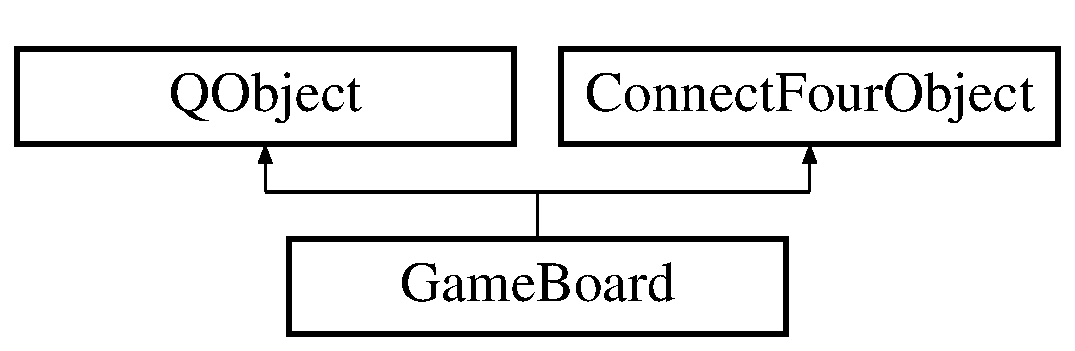
\includegraphics[height=2.000000cm]{class_game_board}
\end{center}
\end{figure}
\subsection*{Public Member Functions}
\begin{DoxyCompactItemize}
\item 
\hypertarget{class_game_board_ae9975214e1b9b33c8d796937aa42520e}{{\bfseries Game\-Board} (int rows, int columns, Q\-Object $\ast$parent=0)}\label{class_game_board_ae9975214e1b9b33c8d796937aa42520e}

\item 
\hypertarget{class_game_board_ac3f19f16873e19e03d56b06ced39792c}{{\bfseries Game\-Board} (const \hyperlink{class_game_board}{Game\-Board} \&other)}\label{class_game_board_ac3f19f16873e19e03d56b06ced39792c}

\item 
bool \hyperlink{class_game_board_a706ae720beb9de8147298676dc75283c}{add\-Coin} (int column, Coin coin)
\begin{DoxyCompactList}\small\item\em add coin to the game board at the specific column \end{DoxyCompactList}\item 
\hypertarget{class_game_board_a99daa5b67393b74abddfd293b17a2acb}{void {\bfseries remove\-Coin} (int column)}\label{class_game_board_a99daa5b67393b74abddfd293b17a2acb}

\item 
\hypertarget{class_game_board_a72290b30d47b27d1a929150cd9d16305}{Result \hyperlink{class_game_board_a72290b30d47b27d1a929150cd9d16305}{check\-Game\-Conditions} ()}\label{class_game_board_a72290b30d47b27d1a929150cd9d16305}

\begin{DoxyCompactList}\small\item\em check if the game is over \end{DoxyCompactList}\item 
\hypertarget{class_game_board_ad2c44e434b52ccb41d4b272b498cbbac}{std\-::vector$<$ int $>$ \hyperlink{class_game_board_ad2c44e434b52ccb41d4b272b498cbbac}{get\-Available\-Moves} ()}\label{class_game_board_ad2c44e434b52ccb41d4b272b498cbbac}

\begin{DoxyCompactList}\small\item\em returns list of available columns \end{DoxyCompactList}\item 
\hypertarget{class_game_board_ae90c2043ae979dc35dea08113bac278a}{std\-::vector$<$ std\-::shared\-\_\-ptr\\*
$<$ \hyperlink{class_board_column}{Board\-Column} $>$ $>$ {\bfseries get\-Current\-Board} ()}\label{class_game_board_ae90c2043ae979dc35dea08113bac278a}

\item 
\hypertarget{class_game_board_ad533f495fa4f39c15e1164a1a5bb702e}{Q\-String {\bfseries serialize} ()}\label{class_game_board_ad533f495fa4f39c15e1164a1a5bb702e}

\item 
\hypertarget{class_game_board_abfd027ca1bf36698290855faff44d1a3}{void {\bfseries deserialize} (Q\-String board)}\label{class_game_board_abfd027ca1bf36698290855faff44d1a3}

\end{DoxyCompactItemize}
\subsection*{Protected Member Functions}
\begin{DoxyCompactItemize}
\item 
\hypertarget{class_game_board_a9d39bb64647af701a265251624287807}{bool {\bfseries check\-Draw\-Conditions} ()}\label{class_game_board_a9d39bb64647af701a265251624287807}

\item 
\hypertarget{class_game_board_a2ac14f3ff1d653e086136792fe0933d6}{Coin {\bfseries check\-Win\-Conditions} ()}\label{class_game_board_a2ac14f3ff1d653e086136792fe0933d6}

\item 
\hypertarget{class_game_board_a15b19b2ec1e4c63b47e113aba42d3ae3}{Coin {\bfseries get\-Coin} (int column, int row)}\label{class_game_board_a15b19b2ec1e4c63b47e113aba42d3ae3}

\item 
\hypertarget{class_game_board_ae43c300f4bc9df8a8d65231f96d335dd}{bool {\bfseries is\-Coin\-Valid\-At} (int column, int row)}\label{class_game_board_ae43c300f4bc9df8a8d65231f96d335dd}

\end{DoxyCompactItemize}
\subsection*{Protected Attributes}
\begin{DoxyCompactItemize}
\item 
\hypertarget{class_game_board_a62a11c93b4a0af85d3613351ac323485}{std\-::vector$<$ std\-::shared\-\_\-ptr\\*
$<$ \hyperlink{class_board_column}{Board\-Column} $>$ $>$ {\bfseries m\-\_\-p\-Game\-Board}}\label{class_game_board_a62a11c93b4a0af85d3613351ac323485}

\end{DoxyCompactItemize}


\subsection{Detailed Description}


Definition at line 16 of file gameboard.\-h.



\subsection{Member Function Documentation}
\hypertarget{class_game_board_a706ae720beb9de8147298676dc75283c}{\index{Game\-Board@{Game\-Board}!add\-Coin@{add\-Coin}}
\index{add\-Coin@{add\-Coin}!GameBoard@{Game\-Board}}
\subsubsection[{add\-Coin}]{\setlength{\rightskip}{0pt plus 5cm}bool Game\-Board\-::add\-Coin (
\begin{DoxyParamCaption}
\item[{int}]{column, }
\item[{Coin}]{coin}
\end{DoxyParamCaption}
)}}\label{class_game_board_a706ae720beb9de8147298676dc75283c}


add coin to the game board at the specific column 


\begin{DoxyParams}{Parameters}
{\em column} & the column where the coin should be added \\
\hline
{\em the} & coin to add \\
\hline
\end{DoxyParams}


Definition at line 21 of file gameboard.\-cpp.



The documentation for this class was generated from the following files\-:\begin{DoxyCompactItemize}
\item 
gameboard.\-h\item 
gameboard.\-cpp\end{DoxyCompactItemize}

\hypertarget{class_game_board_renderer}{\section{Game\-Board\-Renderer Class Reference}
\label{class_game_board_renderer}\index{Game\-Board\-Renderer@{Game\-Board\-Renderer}}
}


Class that is responsible for rendering the gameboard.  




{\ttfamily \#include $<$gameboardrenderer.\-h$>$}

Inheritance diagram for Game\-Board\-Renderer\-:\begin{figure}[H]
\begin{center}
\leavevmode
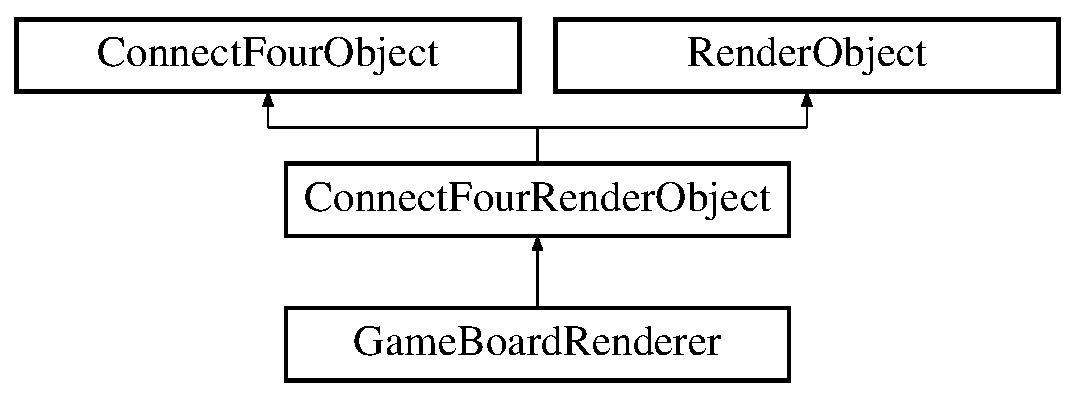
\includegraphics[height=3.000000cm]{class_game_board_renderer}
\end{center}
\end{figure}
\subsection*{Public Member Functions}
\begin{DoxyCompactItemize}
\item 
\hypertarget{class_game_board_renderer_a7bf3a6244010672355b3695fec8547c9}{{\bfseries Game\-Board\-Renderer} (int width, int height, float cell\-Size, Design design)}\label{class_game_board_renderer_a7bf3a6244010672355b3695fec8547c9}

\item 
\hypertarget{class_game_board_renderer_a5b45052cf71976461b07721195dd5dbe}{void {\bfseries init} ()}\label{class_game_board_renderer_a5b45052cf71976461b07721195dd5dbe}

\item 
\hypertarget{class_game_board_renderer_a9daf708f14cd6accf1e2f4cc54bb7d56}{void {\bfseries draw} ()}\label{class_game_board_renderer_a9daf708f14cd6accf1e2f4cc54bb7d56}

\item 
\hypertarget{class_game_board_renderer_a816b3c402bf466641681ed67cefe1041}{int {\bfseries calculate\-And\-Set\-Column\-From\-Mouse\-Point} (Q\-Point point)}\label{class_game_board_renderer_a816b3c402bf466641681ed67cefe1041}

\item 
\hypertarget{class_game_board_renderer_a5678cf7626743de3844406465ca2bf6f}{void {\bfseries set\-Current\-Active\-Player} (Coin player)}\label{class_game_board_renderer_a5678cf7626743de3844406465ca2bf6f}

\end{DoxyCompactItemize}
\subsection*{Additional Inherited Members}


\subsection{Detailed Description}
Class that is responsible for rendering the gameboard. 

Definition at line 13 of file gameboardrenderer.\-h.



The documentation for this class was generated from the following files\-:\begin{DoxyCompactItemize}
\item 
gameboardrenderer.\-h\item 
gameboardrenderer.\-cpp\end{DoxyCompactItemize}

\hypertarget{class_game_client}{\section{Game\-Client Class Reference}
\label{class_game_client}\index{Game\-Client@{Game\-Client}}
}


Class that handles the client network object.  




{\ttfamily \#include $<$gameclient.\-h$>$}

Inheritance diagram for Game\-Client\-:\begin{figure}[H]
\begin{center}
\leavevmode
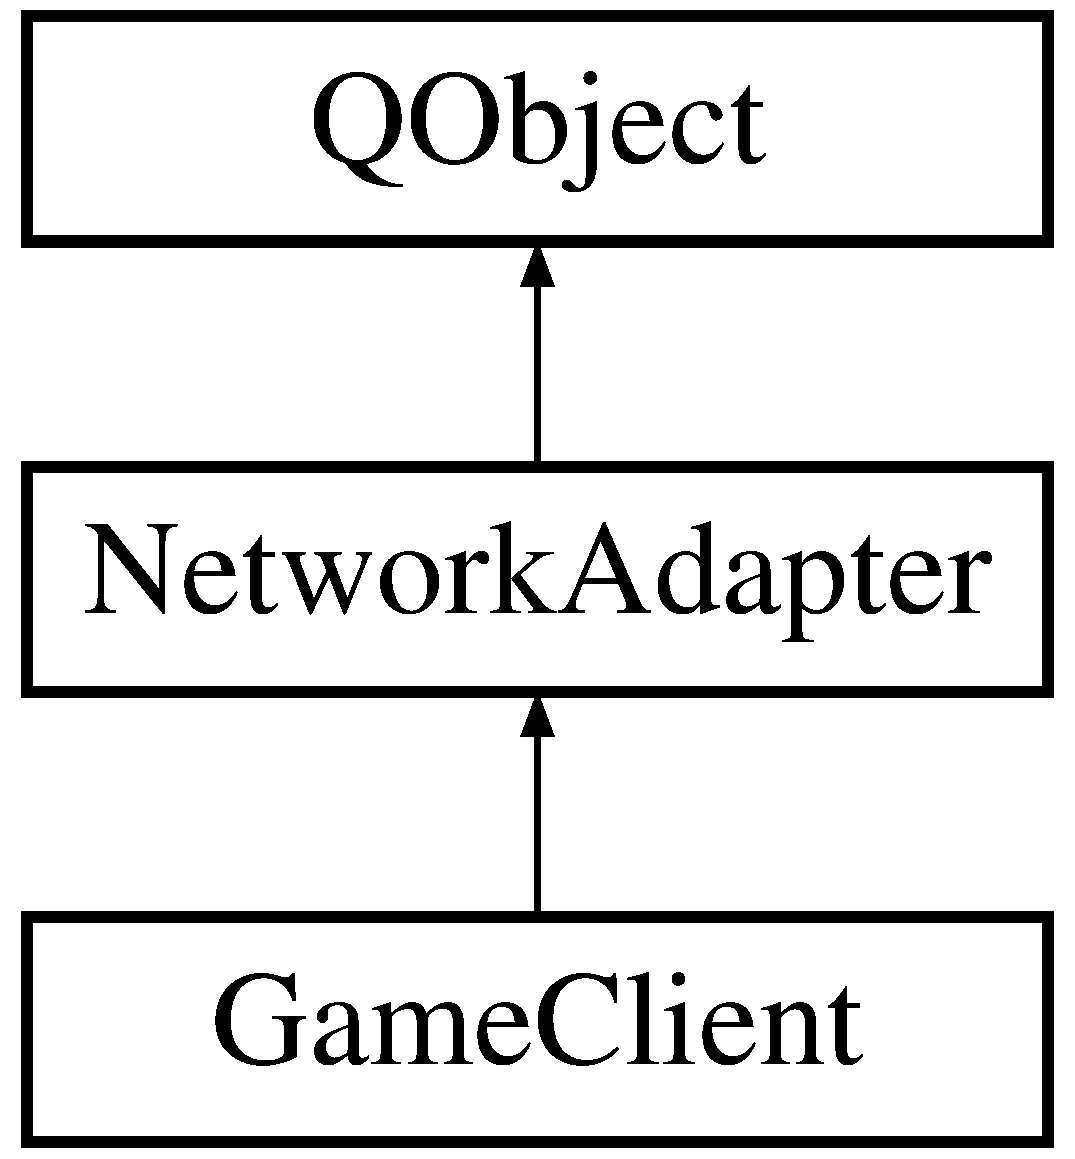
\includegraphics[height=3.000000cm]{class_game_client}
\end{center}
\end{figure}
\subsection*{Public Slots}
\begin{DoxyCompactItemize}
\item 
\hypertarget{class_game_client_aac63bd682b0cfde980b042bf8145e883}{void \hyperlink{class_game_client_aac63bd682b0cfde980b042bf8145e883}{connected} ()}\label{class_game_client_aac63bd682b0cfde980b042bf8145e883}

\begin{DoxyCompactList}\small\item\em called when connected to the server \end{DoxyCompactList}\item 
\hypertarget{class_game_client_a0a9f1d81df966a4c3955f6a95b056c0e}{void \hyperlink{class_game_client_a0a9f1d81df966a4c3955f6a95b056c0e}{disconnected} ()}\label{class_game_client_a0a9f1d81df966a4c3955f6a95b056c0e}

\begin{DoxyCompactList}\small\item\em called when disconnected from the server \end{DoxyCompactList}\item 
\hypertarget{class_game_client_a5457bdb6b9a17067bbb67a2498ee395d}{void \hyperlink{class_game_client_a5457bdb6b9a17067bbb67a2498ee395d}{read\-Ready} ()}\label{class_game_client_a5457bdb6b9a17067bbb67a2498ee395d}

\begin{DoxyCompactList}\small\item\em called when new data is available from the client \end{DoxyCompactList}\item 
\hypertarget{class_game_client_a65b0e61165542bee701778b54f212afd}{void {\bfseries refused\-Connection} ()}\label{class_game_client_a65b0e61165542bee701778b54f212afd}

\end{DoxyCompactItemize}
\subsection*{Public Member Functions}
\begin{DoxyCompactItemize}
\item 
\hypertarget{class_game_client_a6c6faf6d8e0524f9b75041b3eaeb718d}{{\bfseries Game\-Client} (Q\-String ip\-Address, Q\-Object $\ast$parent=0)}\label{class_game_client_a6c6faf6d8e0524f9b75041b3eaeb718d}

\item 
\hypertarget{class_game_client_a96c861f5f70e645a28cf6e7a042dfc9f}{void {\bfseries init} ()}\label{class_game_client_a96c861f5f70e645a28cf6e7a042dfc9f}

\item 
\hypertarget{class_game_client_ad6130cb3cddc509730c948e0177c1be2}{void {\bfseries send} (Q\-String data)}\label{class_game_client_ad6130cb3cddc509730c948e0177c1be2}

\end{DoxyCompactItemize}
\subsection*{Additional Inherited Members}


\subsection{Detailed Description}
Class that handles the client network object. 

Definition at line 10 of file gameclient.\-h.



The documentation for this class was generated from the following files\-:\begin{DoxyCompactItemize}
\item 
gameclient.\-h\item 
gameclient.\-cpp\end{DoxyCompactItemize}

\hypertarget{class_game_coin_renderer}{\section{Game\-Coin\-Renderer Class Reference}
\label{class_game_coin_renderer}\index{Game\-Coin\-Renderer@{Game\-Coin\-Renderer}}
}


Class that is responsible for rendering the coins added to the board.  




{\ttfamily \#include $<$gamecoinrenderer.\-h$>$}

Inheritance diagram for Game\-Coin\-Renderer\-:\begin{figure}[H]
\begin{center}
\leavevmode
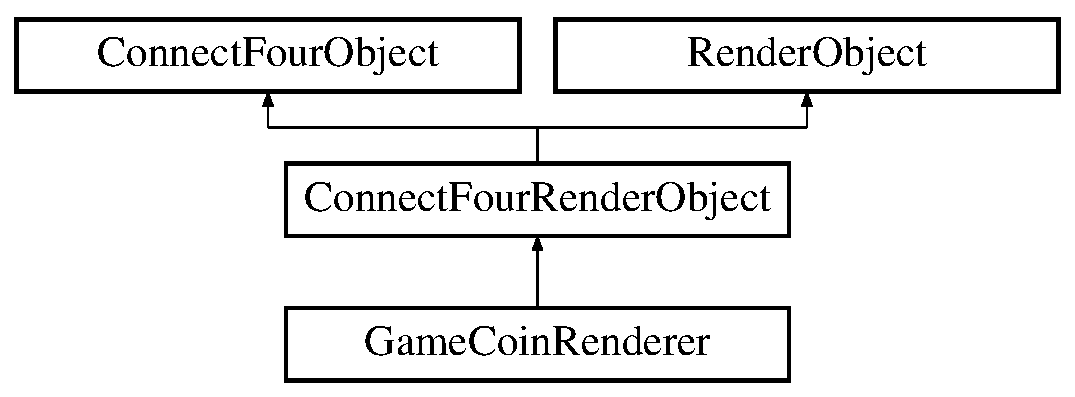
\includegraphics[height=3.000000cm]{class_game_coin_renderer}
\end{center}
\end{figure}
\subsection*{Public Member Functions}
\begin{DoxyCompactItemize}
\item 
\hypertarget{class_game_coin_renderer_a3426566e0d906524729672836c86f5d2}{{\bfseries Game\-Coin\-Renderer} (int width, int height, float cell\-Size, Design design)}\label{class_game_coin_renderer_a3426566e0d906524729672836c86f5d2}

\item 
\hypertarget{class_game_coin_renderer_a2b1b51d93a38675ee1f30fc6cacbaccd}{virtual void \hyperlink{class_game_coin_renderer_a2b1b51d93a38675ee1f30fc6cacbaccd}{draw} ()}\label{class_game_coin_renderer_a2b1b51d93a38675ee1f30fc6cacbaccd}

\begin{DoxyCompactList}\small\item\em renders the board \end{DoxyCompactList}\item 
\hypertarget{class_game_coin_renderer_a88ecbeec05a81381ee676463fe2aac53}{void \hyperlink{class_game_coin_renderer_a88ecbeec05a81381ee676463fe2aac53}{update\-Game\-Coins} (int column, Coin coin)}\label{class_game_coin_renderer_a88ecbeec05a81381ee676463fe2aac53}

\begin{DoxyCompactList}\small\item\em adds coins to the board \end{DoxyCompactList}\item 
\hypertarget{class_game_coin_renderer_a20a3e2499f4f1656a3e1012ef34e7e89}{void \hyperlink{class_game_coin_renderer_a20a3e2499f4f1656a3e1012ef34e7e89}{set\-Game\-Board} (std\-::vector$<$ std\-::shared\-\_\-ptr$<$ \hyperlink{class_board_column}{Board\-Column} $>$ $>$ board)}\label{class_game_coin_renderer_a20a3e2499f4f1656a3e1012ef34e7e89}

\begin{DoxyCompactList}\small\item\em updates the whole board \end{DoxyCompactList}\end{DoxyCompactItemize}
\subsection*{Additional Inherited Members}


\subsection{Detailed Description}
Class that is responsible for rendering the coins added to the board. 

Definition at line 15 of file gamecoinrenderer.\-h.



The documentation for this class was generated from the following files\-:\begin{DoxyCompactItemize}
\item 
gamecoinrenderer.\-h\item 
gamecoinrenderer.\-cpp\end{DoxyCompactItemize}

\hypertarget{class_game_database}{\section{Game\-Database Class Reference}
\label{class_game_database}\index{Game\-Database@{Game\-Database}}
}


singleton class that manages the game result database  




{\ttfamily \#include $<$gamedatabase.\-h$>$}

Inheritance diagram for Game\-Database\-:\begin{figure}[H]
\begin{center}
\leavevmode
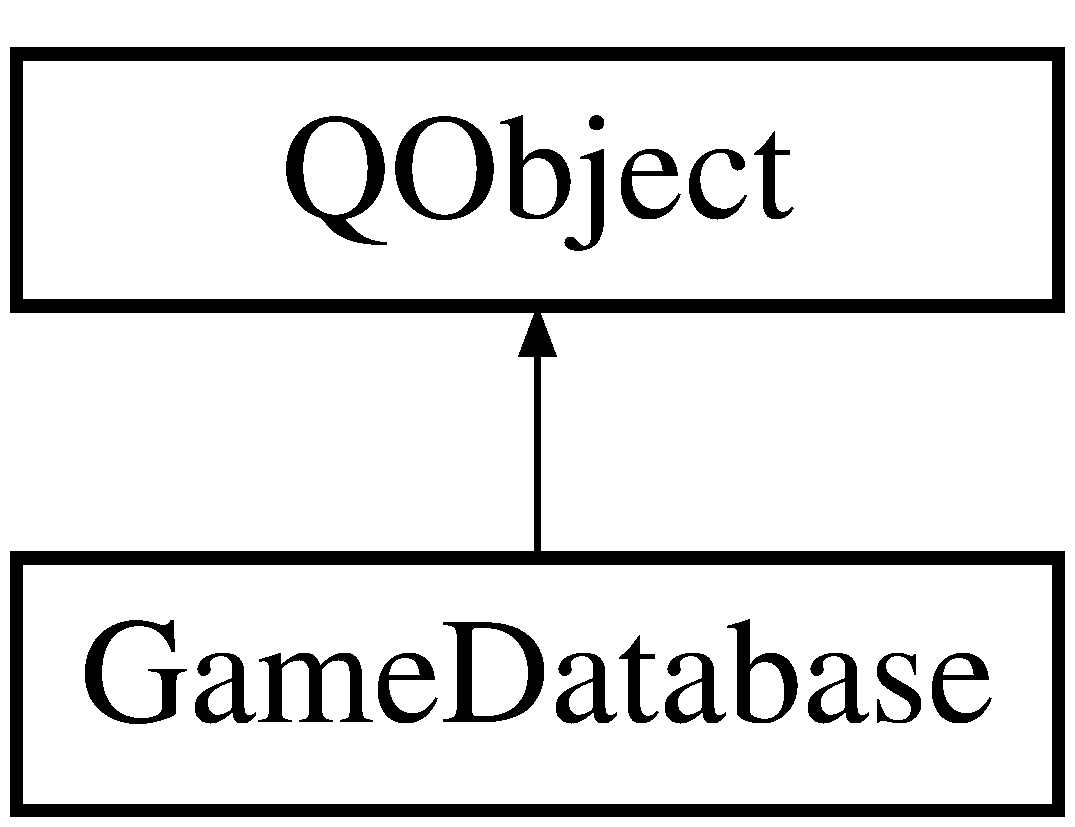
\includegraphics[height=2.000000cm]{class_game_database}
\end{center}
\end{figure}
\subsection*{Public Member Functions}
\begin{DoxyCompactItemize}
\item 
void \hyperlink{class_game_database_aa2e298187a235ff09b53444b65ef806c}{add\-Game} (\hyperlink{struct_game}{Game} game)
\begin{DoxyCompactList}\small\item\em Adds a game to the database. \end{DoxyCompactList}\item 
std\-::vector$<$ std\-::string $>$ \hyperlink{class_game_database_acbcc841f220b5865046d19f8b0e814ed}{get\-Games} ()
\begin{DoxyCompactList}\small\item\em \hyperlink{class_game_database_acbcc841f220b5865046d19f8b0e814ed}{Game\-Database\-::get\-Games} returns all played games that are stored in the sql database. \end{DoxyCompactList}\end{DoxyCompactItemize}
\subsection*{Static Public Member Functions}
\begin{DoxyCompactItemize}
\item 
\hypertarget{class_game_database_a216477b314b74b86d42c943b359ac33a}{static \hyperlink{class_game_database}{Game\-Database} \& {\bfseries get\-Instance} ()}\label{class_game_database_a216477b314b74b86d42c943b359ac33a}

\end{DoxyCompactItemize}


\subsection{Detailed Description}
singleton class that manages the game result database 

Definition at line 13 of file gamedatabase.\-h.



\subsection{Member Function Documentation}
\hypertarget{class_game_database_aa2e298187a235ff09b53444b65ef806c}{\index{Game\-Database@{Game\-Database}!add\-Game@{add\-Game}}
\index{add\-Game@{add\-Game}!GameDatabase@{Game\-Database}}
\subsubsection[{add\-Game}]{\setlength{\rightskip}{0pt plus 5cm}void Game\-Database\-::add\-Game (
\begin{DoxyParamCaption}
\item[{{\bf Game}}]{game}
\end{DoxyParamCaption}
)}}\label{class_game_database_aa2e298187a235ff09b53444b65ef806c}


Adds a game to the database. 


\begin{DoxyParams}{Parameters}
{\em the} & game to add \\
\hline
\end{DoxyParams}


Definition at line 32 of file gamedatabase.\-cpp.

\hypertarget{class_game_database_acbcc841f220b5865046d19f8b0e814ed}{\index{Game\-Database@{Game\-Database}!get\-Games@{get\-Games}}
\index{get\-Games@{get\-Games}!GameDatabase@{Game\-Database}}
\subsubsection[{get\-Games}]{\setlength{\rightskip}{0pt plus 5cm}std\-::vector$<$ std\-::string $>$ Game\-Database\-::get\-Games (
\begin{DoxyParamCaption}
{}
\end{DoxyParamCaption}
)}}\label{class_game_database_acbcc841f220b5865046d19f8b0e814ed}


\hyperlink{class_game_database_acbcc841f220b5865046d19f8b0e814ed}{Game\-Database\-::get\-Games} returns all played games that are stored in the sql database. 

Return played games \begin{DoxyReturn}{Returns}
the list of games stored in the sql database 
\end{DoxyReturn}


Definition at line 57 of file gamedatabase.\-cpp.



The documentation for this class was generated from the following files\-:\begin{DoxyCompactItemize}
\item 
gamedatabase.\-h\item 
gamedatabase.\-cpp\end{DoxyCompactItemize}

\hypertarget{class_game_manager}{\section{Game\-Manager Class Reference}
\label{class_game_manager}\index{Game\-Manager@{Game\-Manager}}
}


Class that handles game states and instanciates renderer and board.  




{\ttfamily \#include $<$gamemanager.\-h$>$}

Inheritance diagram for Game\-Manager\-:\begin{figure}[H]
\begin{center}
\leavevmode
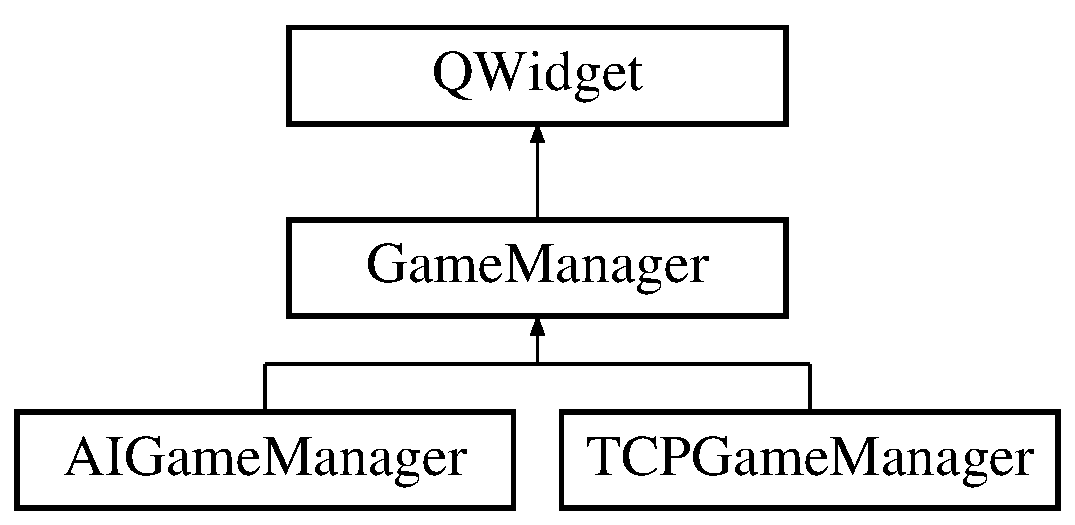
\includegraphics[height=3.000000cm]{class_game_manager}
\end{center}
\end{figure}
\subsection*{Public Slots}
\begin{DoxyCompactItemize}
\item 
\hypertarget{class_game_manager_a55876082b15630acf8109b5f0a33e6bd}{void {\bfseries game\-End} ()}\label{class_game_manager_a55876082b15630acf8109b5f0a33e6bd}

\item 
\hypertarget{class_game_manager_a7ecc3a14cd9e92f50729b37d1364953f}{void \hyperlink{class_game_manager_a7ecc3a14cd9e92f50729b37d1364953f}{update} ()}\label{class_game_manager_a7ecc3a14cd9e92f50729b37d1364953f}

\begin{DoxyCompactList}\small\item\em poll mouse position and update states \end{DoxyCompactList}\item 
\hypertarget{class_game_manager_ac15bf5701604781f66047dc8c94f70a7}{void \hyperlink{class_game_manager_ac15bf5701604781f66047dc8c94f70a7}{mouse\-Press\-Event} (Q\-Mouse\-Event $\ast$event)}\label{class_game_manager_ac15bf5701604781f66047dc8c94f70a7}

\begin{DoxyCompactList}\small\item\em drop coins and check finish game \end{DoxyCompactList}\item 
\hypertarget{class_game_manager_a452f27d846213676394663c8d223983d}{void {\bfseries save\-Game} ()}\label{class_game_manager_a452f27d846213676394663c8d223983d}

\item 
\hypertarget{class_game_manager_ad7e262dd756247130c085ead21b34d87}{void \hyperlink{class_game_manager_ad7e262dd756247130c085ead21b34d87}{load\-Game} (Q\-String game\-Board)}\label{class_game_manager_ad7e262dd756247130c085ead21b34d87}

\begin{DoxyCompactList}\small\item\em also handles start game \end{DoxyCompactList}\item 
\hypertarget{class_game_manager_af49538ffbacf3ed465fe23191f0a7378}{void {\bfseries switch\-Player} ()}\label{class_game_manager_af49538ffbacf3ed465fe23191f0a7378}

\item 
\hypertarget{class_game_manager_aef672bf56ae84eb10a65bf227e487717}{\hyperlink{class_player}{Player} {\bfseries get\-Current\-Active\-Player} ()}\label{class_game_manager_aef672bf56ae84eb10a65bf227e487717}

\item 
\hypertarget{class_game_manager_a875582122292a52ffcae786a46490f89}{\hyperlink{class_player}{Player} {\bfseries get\-Current\-Inactive\-Player} ()}\label{class_game_manager_a875582122292a52ffcae786a46490f89}

\end{DoxyCompactItemize}
\subsection*{Signals}
\begin{DoxyCompactItemize}
\item 
\hypertarget{class_game_manager_ae63cd6e5b6b2458d5260d421433aa43c}{void {\bfseries game\-Started} ()}\label{class_game_manager_ae63cd6e5b6b2458d5260d421433aa43c}

\end{DoxyCompactItemize}
\subsection*{Public Member Functions}
\begin{DoxyCompactItemize}
\item 
\hypertarget{class_game_manager_a22f8d699d465b1246ed1ca95cb5e8126}{{\bfseries Game\-Manager} (Q\-Widget $\ast$parent=0)}\label{class_game_manager_a22f8d699d465b1246ed1ca95cb5e8126}

\item 
\hypertarget{class_game_manager_a4acbc34fa6c280d0f6d48ff867626ce2}{virtual void \hyperlink{class_game_manager_a4acbc34fa6c280d0f6d48ff867626ce2}{start\-Game} (\hyperlink{struct_settings}{Settings} settings)}\label{class_game_manager_a4acbc34fa6c280d0f6d48ff867626ce2}

\begin{DoxyCompactList}\small\item\em instanciates renderer and gameboard \end{DoxyCompactList}\item 
\hypertarget{class_game_manager_a6ec9d87c1a6366be0f5b2191b798a679}{virtual void \hyperlink{class_game_manager_a6ec9d87c1a6366be0f5b2191b798a679}{set\-Starting\-Player} (\hyperlink{struct_settings}{Settings} settings, Coin player=R\-E\-D)}\label{class_game_manager_a6ec9d87c1a6366be0f5b2191b798a679}

\begin{DoxyCompactList}\small\item\em used for diffent game managers to handle starting player \end{DoxyCompactList}\item 
\hypertarget{class_game_manager_afc363c6765b4fdf990f75bd5978a9dbb}{void {\bfseries finish\-Game} (\hyperlink{struct_game}{Game} game)}\label{class_game_manager_afc363c6765b4fdf990f75bd5978a9dbb}

\end{DoxyCompactItemize}
\subsection*{Protected Member Functions}
\begin{DoxyCompactItemize}
\item 
\hypertarget{class_game_manager_a4d65975808a9ddce05814b0708b11268}{void {\bfseries check\-And\-Handle\-Win} (int column)}\label{class_game_manager_a4d65975808a9ddce05814b0708b11268}

\end{DoxyCompactItemize}
\subsection*{Protected Attributes}
\begin{DoxyCompactItemize}
\item 
\hypertarget{class_game_manager_aeb52618cdb82533c22690a269d7e2ab8}{time\-\_\-t {\bfseries m\-\_\-\-Start\-Time}}\label{class_game_manager_aeb52618cdb82533c22690a269d7e2ab8}

\item 
\hypertarget{class_game_manager_aee76ef2de914b2c0934c5b3264426edb}{Q\-H\-Box\-Layout $\ast$ {\bfseries m\-\_\-p\-Main\-Layout}}\label{class_game_manager_aee76ef2de914b2c0934c5b3264426edb}

\item 
\hypertarget{class_game_manager_af15f419d79f18cf1bfb846633fa60ea6}{\hyperlink{class_game_renderer}{Game\-Renderer} $\ast$ {\bfseries m\-\_\-p\-Renderer}}\label{class_game_manager_af15f419d79f18cf1bfb846633fa60ea6}

\item 
\hypertarget{class_game_manager_a9413c0906a485820589ea7c75d9f25b1}{std\-::shared\-\_\-ptr$<$ \hyperlink{class_game_board}{Game\-Board} $>$ {\bfseries m\-\_\-p\-Game\-Board}}\label{class_game_manager_a9413c0906a485820589ea7c75d9f25b1}

\item 
\hypertarget{class_game_manager_a8f611fd41149c74160bf1314d3c8ce09}{\hyperlink{class_game_over_screen}{Game\-Over\-Screen} $\ast$ {\bfseries m\-\_\-p\-Game\-Over\-Screen}}\label{class_game_manager_a8f611fd41149c74160bf1314d3c8ce09}

\item 
\hypertarget{class_game_manager_acc65f12646b0b5f041685066da3d5e7e}{Q\-Timer $\ast$ {\bfseries m\-\_\-p\-Update\-Timer}}\label{class_game_manager_acc65f12646b0b5f041685066da3d5e7e}

\item 
\hypertarget{class_game_manager_a333d215d519fe0789a64c369bdb7a4ee}{\hyperlink{struct_settings}{Settings} {\bfseries m\-\_\-\-Settings}}\label{class_game_manager_a333d215d519fe0789a64c369bdb7a4ee}

\item 
\hypertarget{class_game_manager_a85d58e6dbc954f0441fb5fdb8c797564}{int {\bfseries m\-\_\-\-Current\-Column}}\label{class_game_manager_a85d58e6dbc954f0441fb5fdb8c797564}

\item 
\hypertarget{class_game_manager_a266242aba3c8f5a98b79bd48bf257a5d}{\hyperlink{class_player}{Player} {\bfseries m\-\_\-\-Current\-Player}}\label{class_game_manager_a266242aba3c8f5a98b79bd48bf257a5d}

\item 
\hypertarget{class_game_manager_a354706b4266f9720a284402a2c22b060}{\hyperlink{class_player}{Player} {\bfseries m\-\_\-\-Player1}}\label{class_game_manager_a354706b4266f9720a284402a2c22b060}

\item 
\hypertarget{class_game_manager_a53dc81fe5edc0284d9e15557494d5f17}{\hyperlink{class_player}{Player} {\bfseries m\-\_\-\-Player2}}\label{class_game_manager_a53dc81fe5edc0284d9e15557494d5f17}

\item 
\hypertarget{class_game_manager_aa352a1a6b760aefdc1c21065eb5e1c5b}{bool {\bfseries m\-\_\-\-Current\-Is\-Player1}}\label{class_game_manager_aa352a1a6b760aefdc1c21065eb5e1c5b}

\item 
\hypertarget{class_game_manager_a4357ddc5393953e39d5b217103e85f63}{bool {\bfseries m\-\_\-\-Finished}}\label{class_game_manager_a4357ddc5393953e39d5b217103e85f63}

\end{DoxyCompactItemize}


\subsection{Detailed Description}
Class that handles game states and instanciates renderer and board. 

Definition at line 18 of file gamemanager.\-h.



The documentation for this class was generated from the following files\-:\begin{DoxyCompactItemize}
\item 
gamemanager.\-h\item 
gamemanager.\-cpp\end{DoxyCompactItemize}

\hypertarget{class_game_over_screen}{\section{Game\-Over\-Screen Class Reference}
\label{class_game_over_screen}\index{Game\-Over\-Screen@{Game\-Over\-Screen}}
}
Inheritance diagram for Game\-Over\-Screen\-:\begin{figure}[H]
\begin{center}
\leavevmode
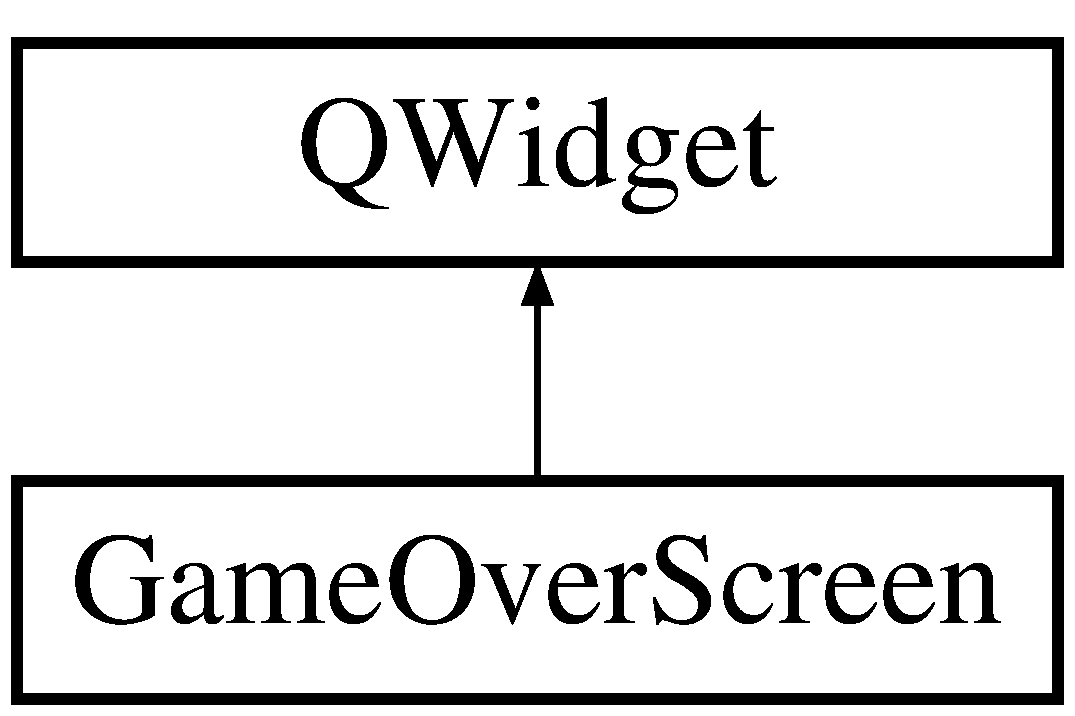
\includegraphics[height=2.000000cm]{class_game_over_screen}
\end{center}
\end{figure}
\subsection*{Public Member Functions}
\begin{DoxyCompactItemize}
\item 
\hypertarget{class_game_over_screen_af87dfa0db651123e3a77265b5c66da13}{{\bfseries Game\-Over\-Screen} (Q\-Widget $\ast$parent=0)}\label{class_game_over_screen_af87dfa0db651123e3a77265b5c66da13}

\item 
\hypertarget{class_game_over_screen_a9767d775fcb476810e1d3690e631aa62}{void {\bfseries set\-Winner} (Q\-String winner)}\label{class_game_over_screen_a9767d775fcb476810e1d3690e631aa62}

\end{DoxyCompactItemize}


\subsection{Detailed Description}


Definition at line 10 of file gameoverscreen.\-h.



The documentation for this class was generated from the following files\-:\begin{DoxyCompactItemize}
\item 
gameoverscreen.\-h\item 
gameoverscreen.\-cpp\end{DoxyCompactItemize}

\hypertarget{class_game_renderer}{\section{Game\-Renderer Class Reference}
\label{class_game_renderer}\index{Game\-Renderer@{Game\-Renderer}}
}


Handles Open\-G\-L window inside main window;.  




{\ttfamily \#include $<$gamerenderer.\-h$>$}

Inheritance diagram for Game\-Renderer\-:\begin{figure}[H]
\begin{center}
\leavevmode
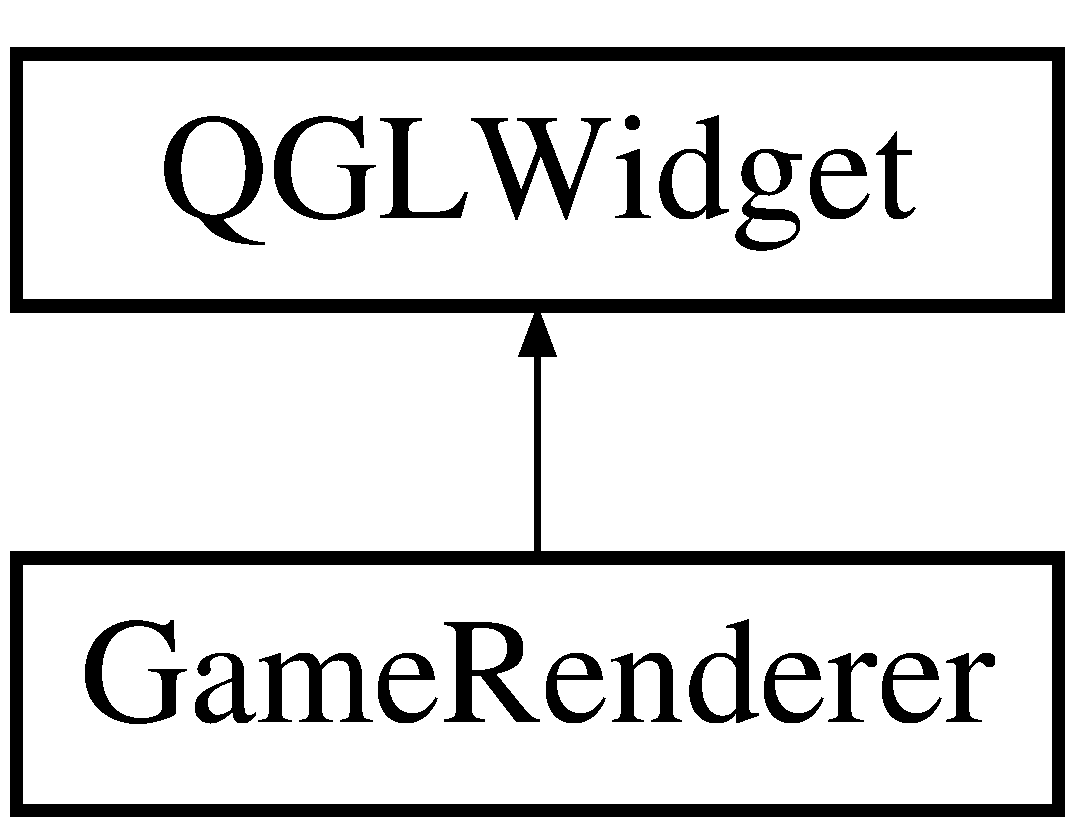
\includegraphics[height=2.000000cm]{class_game_renderer}
\end{center}
\end{figure}
\subsection*{Signals}
\begin{DoxyCompactItemize}
\item 
\hypertarget{class_game_renderer_aff73192b784fa17d2b11c28aa1635f20}{void {\bfseries mouse\-Pressed} (Q\-Mouse\-Event $\ast$event)}\label{class_game_renderer_aff73192b784fa17d2b11c28aa1635f20}

\end{DoxyCompactItemize}
\subsection*{Public Member Functions}
\begin{DoxyCompactItemize}
\item 
\hypertarget{class_game_renderer_a58bc8828909b59c2516549cf3a978f52}{{\bfseries Game\-Renderer} (Q\-Widget $\ast$parent=0)}\label{class_game_renderer_a58bc8828909b59c2516549cf3a978f52}

\item 
\hypertarget{class_game_renderer_a01dc39b34cda656bd5bd72c50103e306}{void {\bfseries initialize} (int width, int height, Design design)}\label{class_game_renderer_a01dc39b34cda656bd5bd72c50103e306}

\item 
\hypertarget{class_game_renderer_af733aa31dd1ace11b9a9b489f5e70573}{void {\bfseries stop} ()}\label{class_game_renderer_af733aa31dd1ace11b9a9b489f5e70573}

\item 
\hypertarget{class_game_renderer_a5a8dc2ad72bfeeebb1f127a5d746dad5}{std\-::shared\-\_\-ptr\\*
$<$ \hyperlink{class_game_board_renderer}{Game\-Board\-Renderer} $>$ {\bfseries get\-Game\-Board\-Renderer} () const }\label{class_game_renderer_a5a8dc2ad72bfeeebb1f127a5d746dad5}

\item 
\hypertarget{class_game_renderer_a28fc9bf401d821351a35f59bf5bd1761}{std\-::shared\-\_\-ptr$<$ \hyperlink{class_game_coin_renderer}{Game\-Coin\-Renderer} $>$ {\bfseries get\-Game\-Coin\-Renderer} () const }\label{class_game_renderer_a28fc9bf401d821351a35f59bf5bd1761}

\end{DoxyCompactItemize}
\subsection*{Protected Member Functions}
\begin{DoxyCompactItemize}
\item 
\hypertarget{class_game_renderer_ada3f9ec6a94622e3942106c35f910c17}{void {\bfseries initialize\-G\-L} ()}\label{class_game_renderer_ada3f9ec6a94622e3942106c35f910c17}

\item 
\hypertarget{class_game_renderer_afe54bbab14adcee6d4a30c2ac74aea84}{void {\bfseries paint\-G\-L} ()}\label{class_game_renderer_afe54bbab14adcee6d4a30c2ac74aea84}

\item 
\hypertarget{class_game_renderer_a96621b18ee77b658ba49ed13085006ab}{void {\bfseries resize\-G\-L} (int width, int height)}\label{class_game_renderer_a96621b18ee77b658ba49ed13085006ab}

\item 
\hypertarget{class_game_renderer_a88c0cc3a0a2ad5dce8ed5f738e8a7dc0}{void {\bfseries mouse\-Press\-Event} (Q\-Mouse\-Event $\ast$event)}\label{class_game_renderer_a88c0cc3a0a2ad5dce8ed5f738e8a7dc0}

\end{DoxyCompactItemize}


\subsection{Detailed Description}
Handles Open\-G\-L window inside main window;. 

Definition at line 54 of file gamerenderer.\-h.



The documentation for this class was generated from the following files\-:\begin{DoxyCompactItemize}
\item 
gamerenderer.\-h\item 
gamerenderer.\-cpp\end{DoxyCompactItemize}

\hypertarget{class_game_results}{\section{Game\-Results Class Reference}
\label{class_game_results}\index{Game\-Results@{Game\-Results}}
}


show previous games  




{\ttfamily \#include $<$gameresults.\-h$>$}

Inheritance diagram for Game\-Results\-:\begin{figure}[H]
\begin{center}
\leavevmode
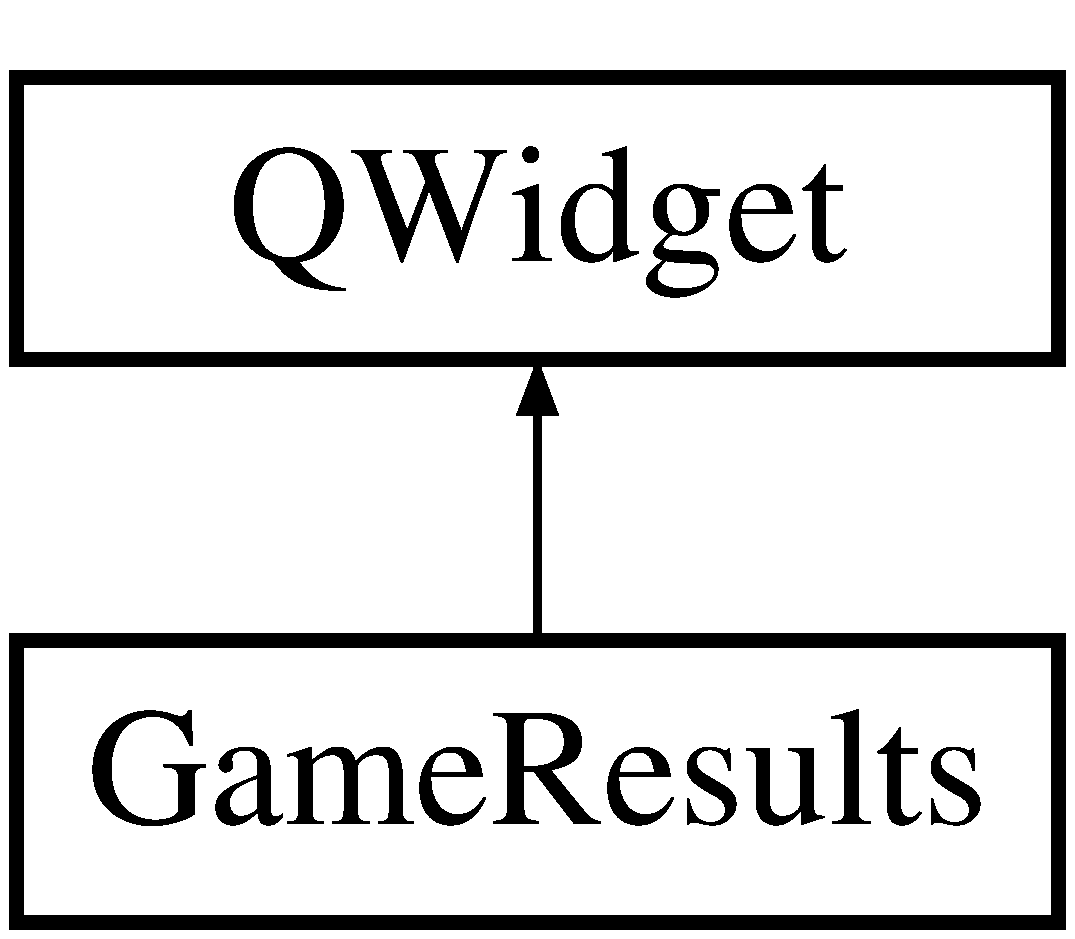
\includegraphics[height=2.000000cm]{class_game_results}
\end{center}
\end{figure}
\subsection*{Public Member Functions}
\begin{DoxyCompactItemize}
\item 
\hypertarget{class_game_results_a1d267b8278b4a65f384a29f2c194cc2c}{{\bfseries Game\-Results} (Q\-Widget $\ast$parent=0)}\label{class_game_results_a1d267b8278b4a65f384a29f2c194cc2c}

\end{DoxyCompactItemize}
\subsection*{Protected Member Functions}
\begin{DoxyCompactItemize}
\item 
\hypertarget{class_game_results_a33935ceabbb695bfdeb955b2a5167448}{void {\bfseries show\-Event} (Q\-Show\-Event $\ast$)}\label{class_game_results_a33935ceabbb695bfdeb955b2a5167448}

\end{DoxyCompactItemize}


\subsection{Detailed Description}
show previous games 

Definition at line 11 of file gameresults.\-h.



The documentation for this class was generated from the following files\-:\begin{DoxyCompactItemize}
\item 
gameresults.\-h\item 
gameresults.\-cpp\end{DoxyCompactItemize}

\hypertarget{class_game_server}{\section{Game\-Server Class Reference}
\label{class_game_server}\index{Game\-Server@{Game\-Server}}
}


Class that handles server client connection.  




{\ttfamily \#include $<$gameserver.\-h$>$}

Inheritance diagram for Game\-Server\-:\begin{figure}[H]
\begin{center}
\leavevmode
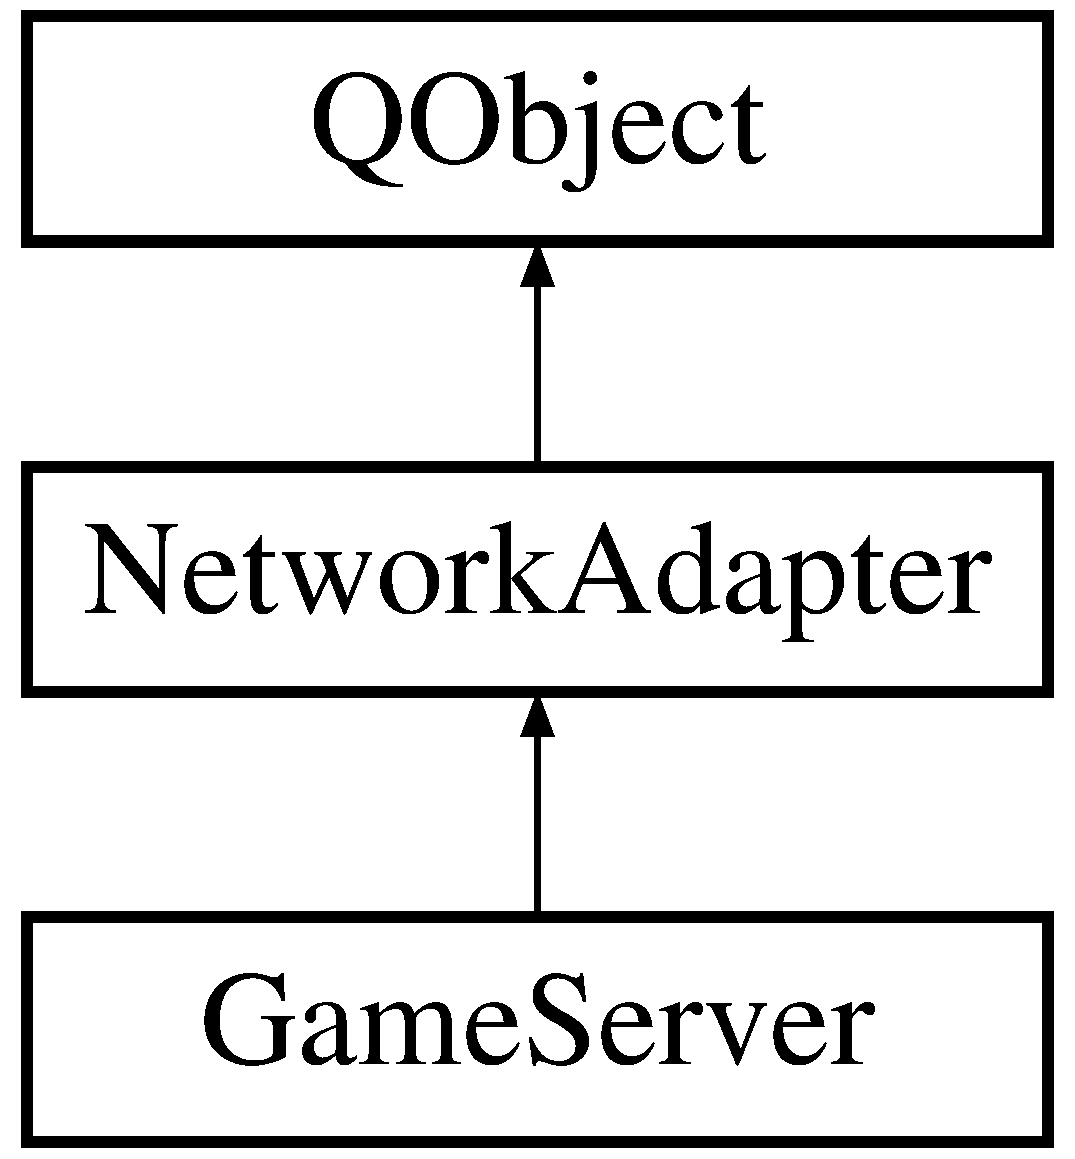
\includegraphics[height=3.000000cm]{class_game_server}
\end{center}
\end{figure}
\subsection*{Public Slots}
\begin{DoxyCompactItemize}
\item 
\hypertarget{class_game_server_ae41954b45bd6e4f7cff0b9c9034206cc}{void \hyperlink{class_game_server_ae41954b45bd6e4f7cff0b9c9034206cc}{new\-Connection} ()}\label{class_game_server_ae41954b45bd6e4f7cff0b9c9034206cc}

\begin{DoxyCompactList}\small\item\em called when a new client connects \end{DoxyCompactList}\item 
\hypertarget{class_game_server_ae04551b358465ca81a34073abb7d6380}{void \hyperlink{class_game_server_ae04551b358465ca81a34073abb7d6380}{read\-Ready} ()}\label{class_game_server_ae04551b358465ca81a34073abb7d6380}

\begin{DoxyCompactList}\small\item\em called when new data is available from the client \end{DoxyCompactList}\end{DoxyCompactItemize}
\subsection*{Public Member Functions}
\begin{DoxyCompactItemize}
\item 
\hypertarget{class_game_server_a23246629b4e19dcd029ad89455147461}{{\bfseries Game\-Server} (Q\-Object $\ast$parent=0)}\label{class_game_server_a23246629b4e19dcd029ad89455147461}

\item 
\hypertarget{class_game_server_a65f06eb193e2ce2670f1b2f65c0a7469}{void {\bfseries init} ()}\label{class_game_server_a65f06eb193e2ce2670f1b2f65c0a7469}

\item 
\hypertarget{class_game_server_a58e009e4c2444745fb86a4085a0ab376}{void {\bfseries send} (Q\-String data)}\label{class_game_server_a58e009e4c2444745fb86a4085a0ab376}

\end{DoxyCompactItemize}
\subsection*{Additional Inherited Members}


\subsection{Detailed Description}
Class that handles server client connection. 

Definition at line 12 of file gameserver.\-h.



The documentation for this class was generated from the following files\-:\begin{DoxyCompactItemize}
\item 
gameserver.\-h\item 
gameserver.\-cpp\end{DoxyCompactItemize}

\hypertarget{class_helper}{\section{Helper Class Reference}
\label{class_helper}\index{Helper@{Helper}}
}


\hyperlink{class_helper}{Helper} class for Connect Four.  




{\ttfamily \#include $<$helper.\-h$>$}

\subsection*{Static Public Member Functions}
\begin{DoxyCompactItemize}
\item 
\hypertarget{class_helper_a63b53176165ddc6d82677009e27334ef}{static Q\-String {\bfseries server\-Search\-Result} ()}\label{class_helper_a63b53176165ddc6d82677009e27334ef}

\item 
\hypertarget{class_helper_a38336498f52ddebd8c711407c0d0504b}{static Q\-String {\bfseries server\-Search\-Request} ()}\label{class_helper_a38336498f52ddebd8c711407c0d0504b}

\item 
\hypertarget{class_helper_a8facbf43c227514834b49391ef476740}{static uint {\bfseries server\-Search\-Port} ()}\label{class_helper_a8facbf43c227514834b49391ef476740}

\item 
\hypertarget{class_helper_a13ac9ee4039795a9b27bc38a81b9f870}{static Q\-String {\bfseries board\-Update} ()}\label{class_helper_a13ac9ee4039795a9b27bc38a81b9f870}

\item 
\hypertarget{class_helper_aae6bf6a7d72c0ec9871fbe7c328236fa}{static Q\-String {\bfseries chat\-Message} ()}\label{class_helper_aae6bf6a7d72c0ec9871fbe7c328236fa}

\item 
\hypertarget{class_helper_ae7ae04b5ed393589228994c9ce203cac}{static void {\bfseries Draw\-Circle} (float radius)}\label{class_helper_ae7ae04b5ed393589228994c9ce203cac}

\item 
\hypertarget{class_helper_aa9b0b92a5842b0daf41108b9940bbe44}{static void {\bfseries Draw\-Triangle} (float size)}\label{class_helper_aa9b0b92a5842b0daf41108b9940bbe44}

\item 
\hypertarget{class_helper_a1624591dac426f4491d28a92e6f4a3ac}{static void {\bfseries Draw\-Square} (float size)}\label{class_helper_a1624591dac426f4491d28a92e6f4a3ac}

\item 
\hypertarget{class_helper_a41d44186f3a08524419153f19aa9b5f2}{static Q\-Color {\bfseries Get\-Coin\-Color} (Coin coin)}\label{class_helper_a41d44186f3a08524419153f19aa9b5f2}

\item 
\hypertarget{class_helper_aeb6829bbdecf8901d143d6a364082919}{static Q\-String {\bfseries Coin\-To\-String} (Coin coin)}\label{class_helper_aeb6829bbdecf8901d143d6a364082919}

\item 
\hypertarget{class_helper_a665cf4e080d1e25199e5545df0cc253c}{static Q\-String {\bfseries Result\-To\-String} (Result game)}\label{class_helper_a665cf4e080d1e25199e5545df0cc253c}

\end{DoxyCompactItemize}


\subsection{Detailed Description}
\hyperlink{class_helper}{Helper} class for Connect Four. 

Definition at line 11 of file helper.\-h.



The documentation for this class was generated from the following file\-:\begin{DoxyCompactItemize}
\item 
helper.\-h\end{DoxyCompactItemize}

\hypertarget{class_main_window}{\section{Main\-Window Class Reference}
\label{class_main_window}\index{Main\-Window@{Main\-Window}}
}
Inheritance diagram for Main\-Window\-:\begin{figure}[H]
\begin{center}
\leavevmode
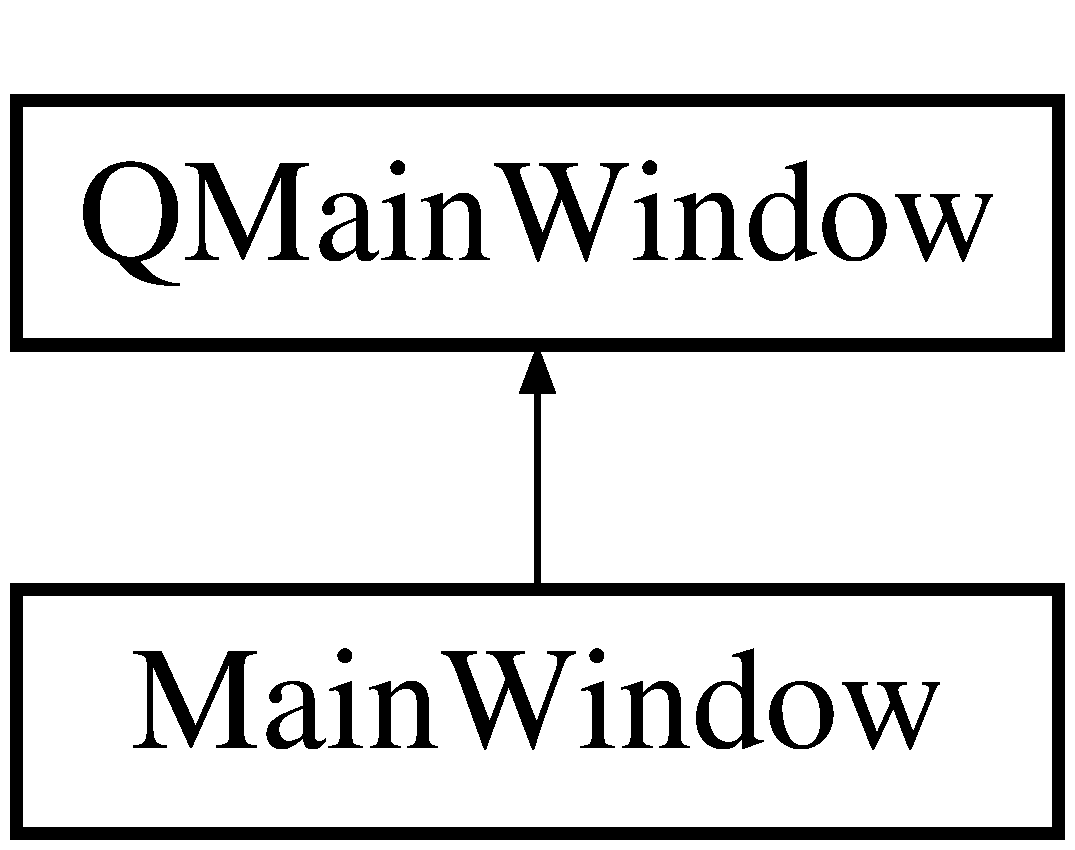
\includegraphics[height=2.000000cm]{class_main_window}
\end{center}
\end{figure}
\subsection*{Public Member Functions}
\begin{DoxyCompactItemize}
\item 
\hypertarget{class_main_window_a8b244be8b7b7db1b08de2a2acb9409db}{{\bfseries Main\-Window} (Q\-Widget $\ast$parent=0)}\label{class_main_window_a8b244be8b7b7db1b08de2a2acb9409db}

\item 
\hypertarget{class_main_window_af747387b0953cbb422b3cb52031b863c}{Q\-Size {\bfseries size} ()}\label{class_main_window_af747387b0953cbb422b3cb52031b863c}

\item 
\hypertarget{class_main_window_a781737f6e3b1f3e97e6a7eebb6396771}{Q\-Size {\bfseries size\-Hint} () const }\label{class_main_window_a781737f6e3b1f3e97e6a7eebb6396771}

\end{DoxyCompactItemize}


\subsection{Detailed Description}


Definition at line 17 of file mainwindow.\-h.



The documentation for this class was generated from the following files\-:\begin{DoxyCompactItemize}
\item 
mainwindow.\-h\item 
mainwindow.\-cpp\end{DoxyCompactItemize}

\hypertarget{class_min_max}{\section{Min\-Max Class Reference}
\label{class_min_max}\index{Min\-Max@{Min\-Max}}
}


Negamax algorithm.  




{\ttfamily \#include $<$minmax.\-h$>$}

\subsection*{Public Member Functions}
\begin{DoxyCompactItemize}
\item 
\hypertarget{class_min_max_ad5d3439e2da6bdec672b4e068c86f219}{{\bfseries Min\-Max} (A\-I\-Strength strength)}\label{class_min_max_ad5d3439e2da6bdec672b4e068c86f219}

\item 
\hypertarget{class_min_max_a0727d40296556cb72e6b147796e9cb06}{int \hyperlink{class_min_max_a0727d40296556cb72e6b147796e9cb06}{calculate\-Move} (\hyperlink{class_game_board}{Game\-Board} \&board, \hyperlink{class_game_manager}{Game\-Manager} \&manager)}\label{class_min_max_a0727d40296556cb72e6b147796e9cb06}

\begin{DoxyCompactList}\small\item\em calculares the ai's next move \end{DoxyCompactList}\end{DoxyCompactItemize}


\subsection{Detailed Description}
Negamax algorithm. 

Definition at line 16 of file minmax.\-h.



The documentation for this class was generated from the following file\-:\begin{DoxyCompactItemize}
\item 
minmax.\-h\end{DoxyCompactItemize}

\hypertarget{class_network_adapter}{\section{Network\-Adapter Class Reference}
\label{class_network_adapter}\index{Network\-Adapter@{Network\-Adapter}}
}


base class for a network connection (server and client)  




{\ttfamily \#include $<$networkadapter.\-h$>$}

Inheritance diagram for Network\-Adapter\-:\begin{figure}[H]
\begin{center}
\leavevmode
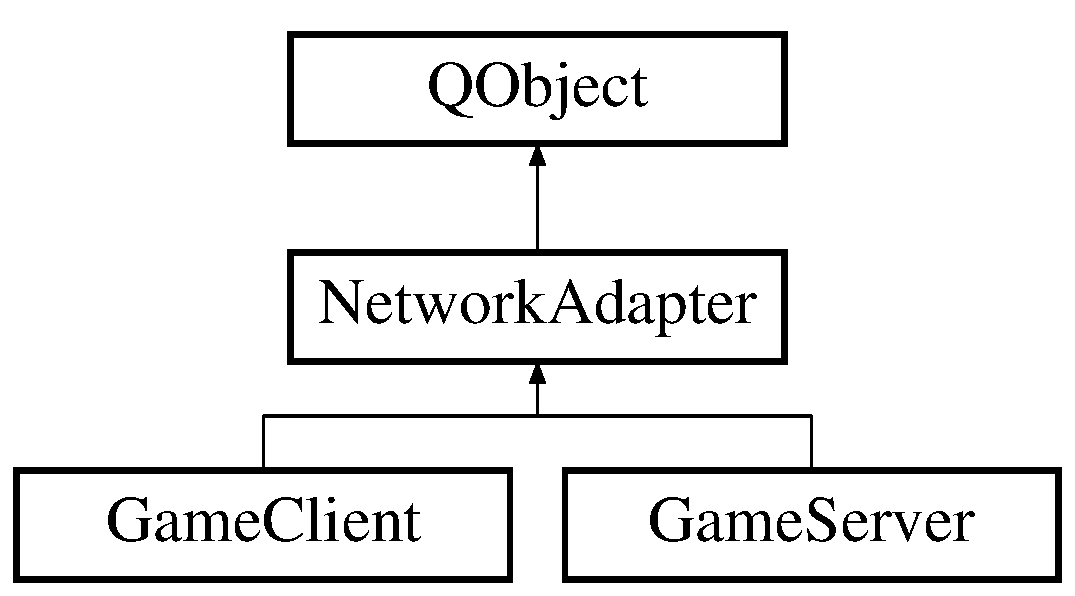
\includegraphics[height=3.000000cm]{class_network_adapter}
\end{center}
\end{figure}
\subsection*{Signals}
\begin{DoxyCompactItemize}
\item 
\hypertarget{class_network_adapter_a2da2230a1cdf125105537d7a5b143bd0}{void \hyperlink{class_network_adapter_a2da2230a1cdf125105537d7a5b143bd0}{connection\-Established} ()}\label{class_network_adapter_a2da2230a1cdf125105537d7a5b143bd0}

\begin{DoxyCompactList}\small\item\em triggered after a new connection has been established either by server or client \end{DoxyCompactList}\item 
\hypertarget{class_network_adapter_ac2e6cce84f774b166dfda66e98ee655e}{void \hyperlink{class_network_adapter_ac2e6cce84f774b166dfda66e98ee655e}{data\-Received} (const Q\-String \&data)}\label{class_network_adapter_ac2e6cce84f774b166dfda66e98ee655e}

\begin{DoxyCompactList}\small\item\em triggered after new data is available on the socket \end{DoxyCompactList}\end{DoxyCompactItemize}
\subsection*{Public Member Functions}
\begin{DoxyCompactItemize}
\item 
\hypertarget{class_network_adapter_a06f7164599740e840ef4663558019319}{{\bfseries Network\-Adapter} (Q\-Object $\ast$parent=0)}\label{class_network_adapter_a06f7164599740e840ef4663558019319}

\item 
\hypertarget{class_network_adapter_a5bfaa6d0344e0026418c99a27548a332}{virtual void {\bfseries init} ()=0}\label{class_network_adapter_a5bfaa6d0344e0026418c99a27548a332}

\item 
\hypertarget{class_network_adapter_a304921c7d4e599031608a9a9217c900f}{virtual void {\bfseries send} (Q\-String data)=0}\label{class_network_adapter_a304921c7d4e599031608a9a9217c900f}

\item 
\hypertarget{class_network_adapter_a955b0bf900e7eca5051c203f86898538}{bool {\bfseries is\-Connected} ()}\label{class_network_adapter_a955b0bf900e7eca5051c203f86898538}

\item 
\hypertarget{class_network_adapter_a37549ba9c99061a8c5407299b380139d}{bool {\bfseries Is\-Server} ()}\label{class_network_adapter_a37549ba9c99061a8c5407299b380139d}

\end{DoxyCompactItemize}
\subsection*{Protected Attributes}
\begin{DoxyCompactItemize}
\item 
\hypertarget{class_network_adapter_a8517d41d27fad01cd65a6342b562f7e0}{bool {\bfseries m\-\_\-\-Is\-Server}}\label{class_network_adapter_a8517d41d27fad01cd65a6342b562f7e0}

\item 
\hypertarget{class_network_adapter_aac7a55e1d924965afcb829f9c9f3da15}{bool {\bfseries m\-\_\-\-Is\-Connected}}\label{class_network_adapter_aac7a55e1d924965afcb829f9c9f3da15}

\item 
\hypertarget{class_network_adapter_a805305b01405a2890d9bbb784d44bde1}{Q\-Tcp\-Socket $\ast$ {\bfseries m\-\_\-p\-Socket}}\label{class_network_adapter_a805305b01405a2890d9bbb784d44bde1}

\end{DoxyCompactItemize}


\subsection{Detailed Description}
base class for a network connection (server and client) 

Definition at line 9 of file networkadapter.\-h.



The documentation for this class was generated from the following files\-:\begin{DoxyCompactItemize}
\item 
networkadapter.\-h\item 
networkadapter.\-cpp\end{DoxyCompactItemize}

\hypertarget{class_player}{\section{Player Class Reference}
\label{class_player}\index{Player@{Player}}
}
\subsection*{Public Member Functions}
\begin{DoxyCompactItemize}
\item 
\hypertarget{class_player_a877063d8943797400d52fe2735d521c3}{{\bfseries Player} (Q\-String name, Coin color, bool is\-Ai\-Player=false)}\label{class_player_a877063d8943797400d52fe2735d521c3}

\item 
\hypertarget{class_player_a60bab4053f47b075a4228b5237394711}{Coin {\bfseries get\-Coin} ()}\label{class_player_a60bab4053f47b075a4228b5237394711}

\item 
\hypertarget{class_player_ade0334ac0e87ac1c5e09ce78f2cafd83}{Q\-String {\bfseries get\-Name} ()}\label{class_player_ade0334ac0e87ac1c5e09ce78f2cafd83}

\item 
\hypertarget{class_player_a0f345ac8c69275c700ed776ddac094c3}{bool {\bfseries is\-Ai\-Player} ()}\label{class_player_a0f345ac8c69275c700ed776ddac094c3}

\end{DoxyCompactItemize}


\subsection{Detailed Description}


Definition at line 7 of file player.\-h.



The documentation for this class was generated from the following file\-:\begin{DoxyCompactItemize}
\item 
player.\-h\end{DoxyCompactItemize}

\hypertarget{class_render_object}{\section{Render\-Object Class Reference}
\label{class_render_object}\index{Render\-Object@{Render\-Object}}
}


abstract class for each renderable object  




{\ttfamily \#include $<$renderobject.\-h$>$}

Inheritance diagram for Render\-Object\-:\begin{figure}[H]
\begin{center}
\leavevmode
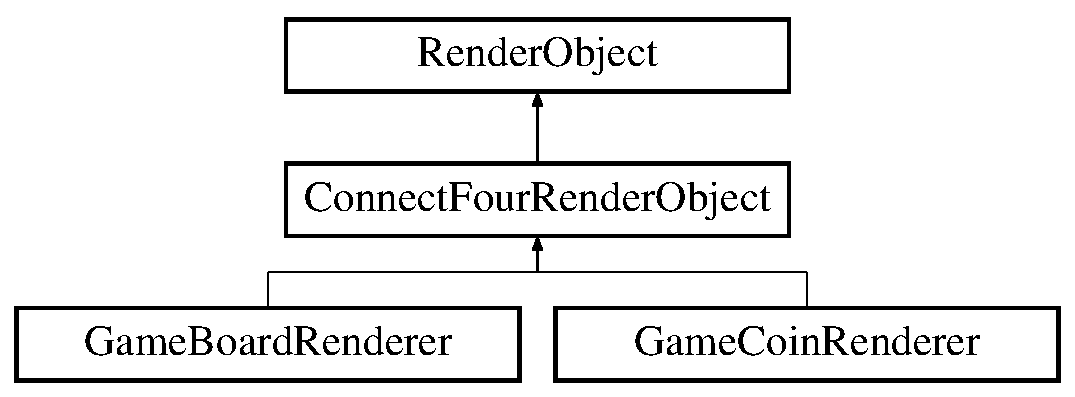
\includegraphics[height=3.000000cm]{class_render_object}
\end{center}
\end{figure}
\subsection*{Public Member Functions}
\begin{DoxyCompactItemize}
\item 
\hypertarget{class_render_object_ac4cc404d2bada4f6652b94cdaa833502}{virtual void {\bfseries init} ()}\label{class_render_object_ac4cc404d2bada4f6652b94cdaa833502}

\item 
\hypertarget{class_render_object_aa4578bf61a73304b8613727cd89ee576}{virtual void {\bfseries draw} ()=0}\label{class_render_object_aa4578bf61a73304b8613727cd89ee576}

\item 
\hypertarget{class_render_object_a46fffcc84648ad62836cab723c8c1f58}{virtual void {\bfseries resize} (int width, int height)=0}\label{class_render_object_a46fffcc84648ad62836cab723c8c1f58}

\end{DoxyCompactItemize}


\subsection{Detailed Description}
abstract class for each renderable object 

Definition at line 5 of file renderobject.\-h.



The documentation for this class was generated from the following file\-:\begin{DoxyCompactItemize}
\item 
renderobject.\-h\end{DoxyCompactItemize}

\hypertarget{class_server_search}{\section{Server\-Search Class Reference}
\label{class_server_search}\index{Server\-Search@{Server\-Search}}
}


The \hyperlink{class_server_search}{Server\-Search} class handles requesting and rendering of a server list in the local network.  




{\ttfamily \#include $<$serversearch.\-h$>$}

Inheritance diagram for Server\-Search\-:\begin{figure}[H]
\begin{center}
\leavevmode
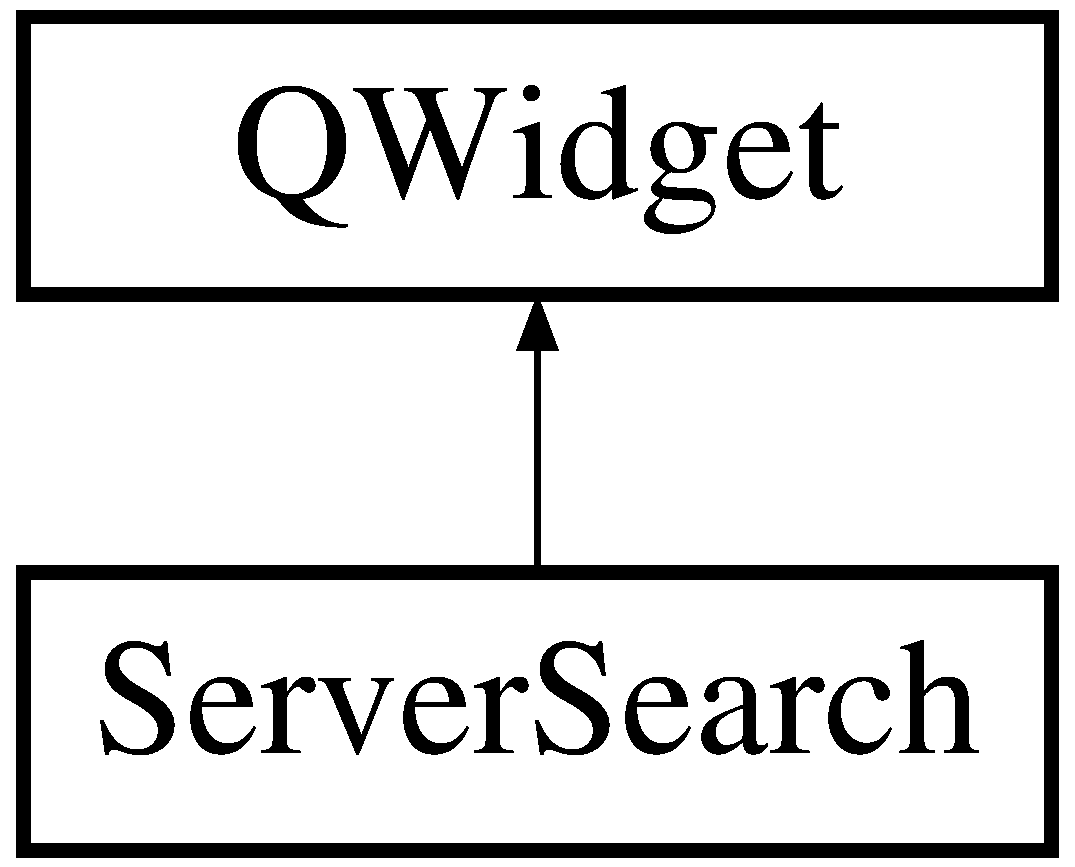
\includegraphics[height=2.000000cm]{class_server_search}
\end{center}
\end{figure}
\subsection*{Public Member Functions}
\begin{DoxyCompactItemize}
\item 
\hypertarget{class_server_search_a53407c1f938da9f6850c4475f292d349}{{\bfseries Server\-Search} (Q\-Widget $\ast$parent=0)}\label{class_server_search_a53407c1f938da9f6850c4475f292d349}

\end{DoxyCompactItemize}
\subsection*{Protected Slots}
\begin{DoxyCompactItemize}
\item 
\hypertarget{class_server_search_a5f0aa647331b434da9e9346100448211}{void \hyperlink{class_server_search_a5f0aa647331b434da9e9346100448211}{read\-Ready} ()}\label{class_server_search_a5f0aa647331b434da9e9346100448211}

\begin{DoxyCompactList}\small\item\em called on response to the serversearch request \end{DoxyCompactList}\end{DoxyCompactItemize}
\subsection*{Protected Member Functions}
\begin{DoxyCompactItemize}
\item 
\hypertarget{class_server_search_a7b9bf3523032f803b44aca2fe27a11dd}{void \hyperlink{class_server_search_a7b9bf3523032f803b44aca2fe27a11dd}{show\-Event} (Q\-Show\-Event $\ast$event)}\label{class_server_search_a7b9bf3523032f803b44aca2fe27a11dd}

\begin{DoxyCompactList}\small\item\em called when the Widget is shown \end{DoxyCompactList}\end{DoxyCompactItemize}


\subsection{Detailed Description}
The \hyperlink{class_server_search}{Server\-Search} class handles requesting and rendering of a server list in the local network. 

Definition at line 18 of file serversearch.\-h.



The documentation for this class was generated from the following files\-:\begin{DoxyCompactItemize}
\item 
serversearch.\-h\item 
serversearch.\-cpp\end{DoxyCompactItemize}

\hypertarget{class_server_search_listener}{\section{Server\-Search\-Listener Class Reference}
\label{class_server_search_listener}\index{Server\-Search\-Listener@{Server\-Search\-Listener}}
}


The \hyperlink{class_server_search_listener}{Server\-Search\-Listener} handles incoming serversearch requests.  




{\ttfamily \#include $<$serversearchlistener.\-h$>$}

Inheritance diagram for Server\-Search\-Listener\-:\begin{figure}[H]
\begin{center}
\leavevmode
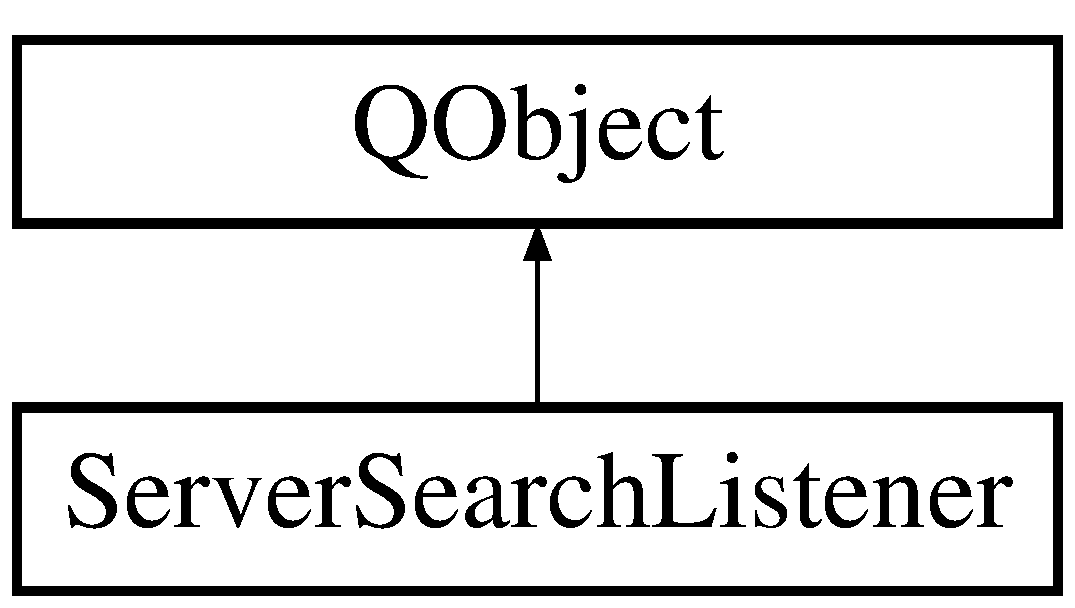
\includegraphics[height=2.000000cm]{class_server_search_listener}
\end{center}
\end{figure}
\subsection*{Public Member Functions}
\begin{DoxyCompactItemize}
\item 
\hypertarget{class_server_search_listener_aa3ee0bdea4c0c4151c3882644e42eb5d}{{\bfseries Server\-Search\-Listener} (Q\-Object $\ast$parent=0)}\label{class_server_search_listener_aa3ee0bdea4c0c4151c3882644e42eb5d}

\end{DoxyCompactItemize}
\subsection*{Protected Slots}
\begin{DoxyCompactItemize}
\item 
\hypertarget{class_server_search_listener_a21a16b4da531df945508189dc7d4d704}{void \hyperlink{class_server_search_listener_a21a16b4da531df945508189dc7d4d704}{process\-Server\-Search\-Request} ()}\label{class_server_search_listener_a21a16b4da531df945508189dc7d4d704}

\begin{DoxyCompactList}\small\item\em process\-Server\-Search\-Request called when new data is available on the socket handles response on the request with sending the first network adapters ip address \end{DoxyCompactList}\end{DoxyCompactItemize}


\subsection{Detailed Description}
The \hyperlink{class_server_search_listener}{Server\-Search\-Listener} handles incoming serversearch requests. 

Definition at line 11 of file serversearchlistener.\-h.



The documentation for this class was generated from the following files\-:\begin{DoxyCompactItemize}
\item 
serversearchlistener.\-h\item 
serversearchlistener.\-cpp\end{DoxyCompactItemize}

\hypertarget{struct_settings}{\section{Settings Struct Reference}
\label{struct_settings}\index{Settings@{Settings}}
}


data holder between ui and game  




{\ttfamily \#include $<$settings.\-h$>$}

\subsection*{Public Attributes}
\begin{DoxyCompactItemize}
\item 
\hypertarget{struct_settings_ac5a707ab0e620e9aeb22d98478197506}{int {\bfseries width}}\label{struct_settings_ac5a707ab0e620e9aeb22d98478197506}

\item 
\hypertarget{struct_settings_af63a2c25f93b1f54a88f9217e95fbcc0}{int {\bfseries height}}\label{struct_settings_af63a2c25f93b1f54a88f9217e95fbcc0}

\item 
\hypertarget{struct_settings_a02c5d891df66d91711d7ef348bc0a98a}{Q\-String {\bfseries player1}}\label{struct_settings_a02c5d891df66d91711d7ef348bc0a98a}

\item 
\hypertarget{struct_settings_af36a424cc1c71f670f4e0b221f1ac2d4}{Q\-String {\bfseries player2}}\label{struct_settings_af36a424cc1c71f670f4e0b221f1ac2d4}

\item 
\hypertarget{struct_settings_a5dd01adc93a126d0c4443b9e04906388}{Q\-String {\bfseries ip\-Address}}\label{struct_settings_a5dd01adc93a126d0c4443b9e04906388}

\item 
\hypertarget{struct_settings_a0d2542ef361af07d3a52243c46305541}{bool {\bfseries use\-A\-I}}\label{struct_settings_a0d2542ef361af07d3a52243c46305541}

\item 
\hypertarget{struct_settings_aa510d772b330cc005608bb764d8aaf2b}{bool {\bfseries ai\-Begins}}\label{struct_settings_aa510d772b330cc005608bb764d8aaf2b}

\item 
\hypertarget{struct_settings_afbfb0309eead50812c931b71fa35289d}{Design {\bfseries design}}\label{struct_settings_afbfb0309eead50812c931b71fa35289d}

\item 
\hypertarget{struct_settings_aa5022e1d185a0f826d2684cd76613090}{A\-I\-Strength {\bfseries ai\-Strength}}\label{struct_settings_aa5022e1d185a0f826d2684cd76613090}

\end{DoxyCompactItemize}


\subsection{Detailed Description}
data holder between ui and game 

Definition at line 21 of file settings.\-h.



The documentation for this struct was generated from the following file\-:\begin{DoxyCompactItemize}
\item 
settings.\-h\end{DoxyCompactItemize}

\hypertarget{class_settings_widget}{\section{Settings\-Widget Class Reference}
\label{class_settings_widget}\index{Settings\-Widget@{Settings\-Widget}}
}
Inheritance diagram for Settings\-Widget\-:\begin{figure}[H]
\begin{center}
\leavevmode
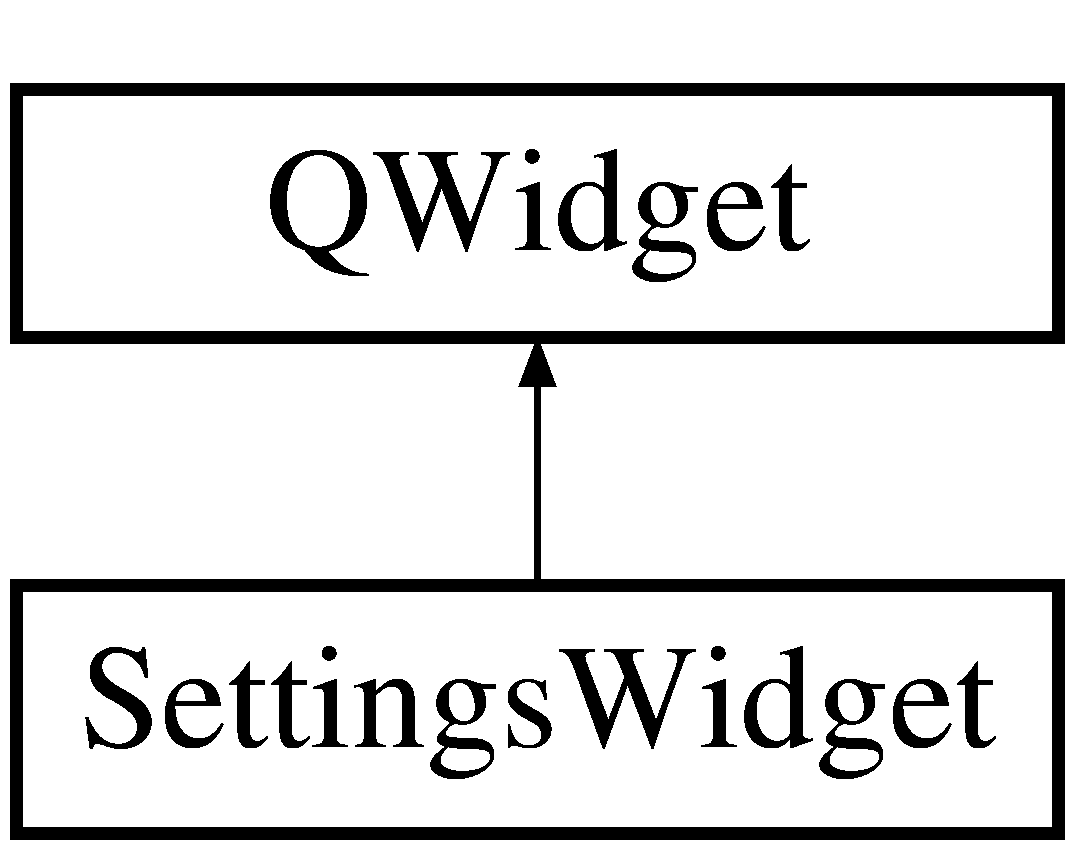
\includegraphics[height=2.000000cm]{class_settings_widget}
\end{center}
\end{figure}
\subsection*{Signals}
\begin{DoxyCompactItemize}
\item 
\hypertarget{class_settings_widget_a0dc3dbbc8b45cae0480cf727ad53c77a}{void {\bfseries start\-Button\-Pressed} (\hyperlink{struct_settings}{Settings} settings)}\label{class_settings_widget_a0dc3dbbc8b45cae0480cf727ad53c77a}

\item 
\hypertarget{class_settings_widget_a3318e4fa37e5fc7aa7b6b272345b9853}{void {\bfseries host\-Server\-Button\-Pressed} (\hyperlink{struct_settings}{Settings} settings)}\label{class_settings_widget_a3318e4fa37e5fc7aa7b6b272345b9853}

\item 
\hypertarget{class_settings_widget_a5d848f32b81af10a30d678816d15fdf4}{void {\bfseries connect\-Button\-Pressed} (\hyperlink{struct_settings}{Settings} settings)}\label{class_settings_widget_a5d848f32b81af10a30d678816d15fdf4}

\item 
\hypertarget{class_settings_widget_a7ee9f48c228d92314768f2e63dcc2b55}{void {\bfseries highscore\-Button\-Pressed} ()}\label{class_settings_widget_a7ee9f48c228d92314768f2e63dcc2b55}

\item 
\hypertarget{class_settings_widget_a30472b488193858a5e1d6205a9f2c14c}{void {\bfseries show\-Chat\-Widget} ()}\label{class_settings_widget_a30472b488193858a5e1d6205a9f2c14c}

\item 
\hypertarget{class_settings_widget_ac8e6df3dc561edb05922fcae047b0074}{void {\bfseries on\-Find\-Server\-Button} ()}\label{class_settings_widget_ac8e6df3dc561edb05922fcae047b0074}

\end{DoxyCompactItemize}
\subsection*{Public Member Functions}
\begin{DoxyCompactItemize}
\item 
\hypertarget{class_settings_widget_ab381a630fcf24d7fe49ab7bd2896c052}{{\bfseries Settings\-Widget} (Q\-Widget $\ast$parent=0)}\label{class_settings_widget_ab381a630fcf24d7fe49ab7bd2896c052}

\end{DoxyCompactItemize}


\subsection{Detailed Description}


Definition at line 11 of file settingswidget.\-h.



The documentation for this class was generated from the following files\-:\begin{DoxyCompactItemize}
\item 
settingswidget.\-h\item 
settingswidget.\-cpp\end{DoxyCompactItemize}

\hypertarget{class_t_c_p_game_manager}{\section{T\-C\-P\-Game\-Manager Class Reference}
\label{class_t_c_p_game_manager}\index{T\-C\-P\-Game\-Manager@{T\-C\-P\-Game\-Manager}}
}


Gamemanager that handles Network game related tasks.  




{\ttfamily \#include $<$tcpgamemanager.\-h$>$}

Inheritance diagram for T\-C\-P\-Game\-Manager\-:\begin{figure}[H]
\begin{center}
\leavevmode
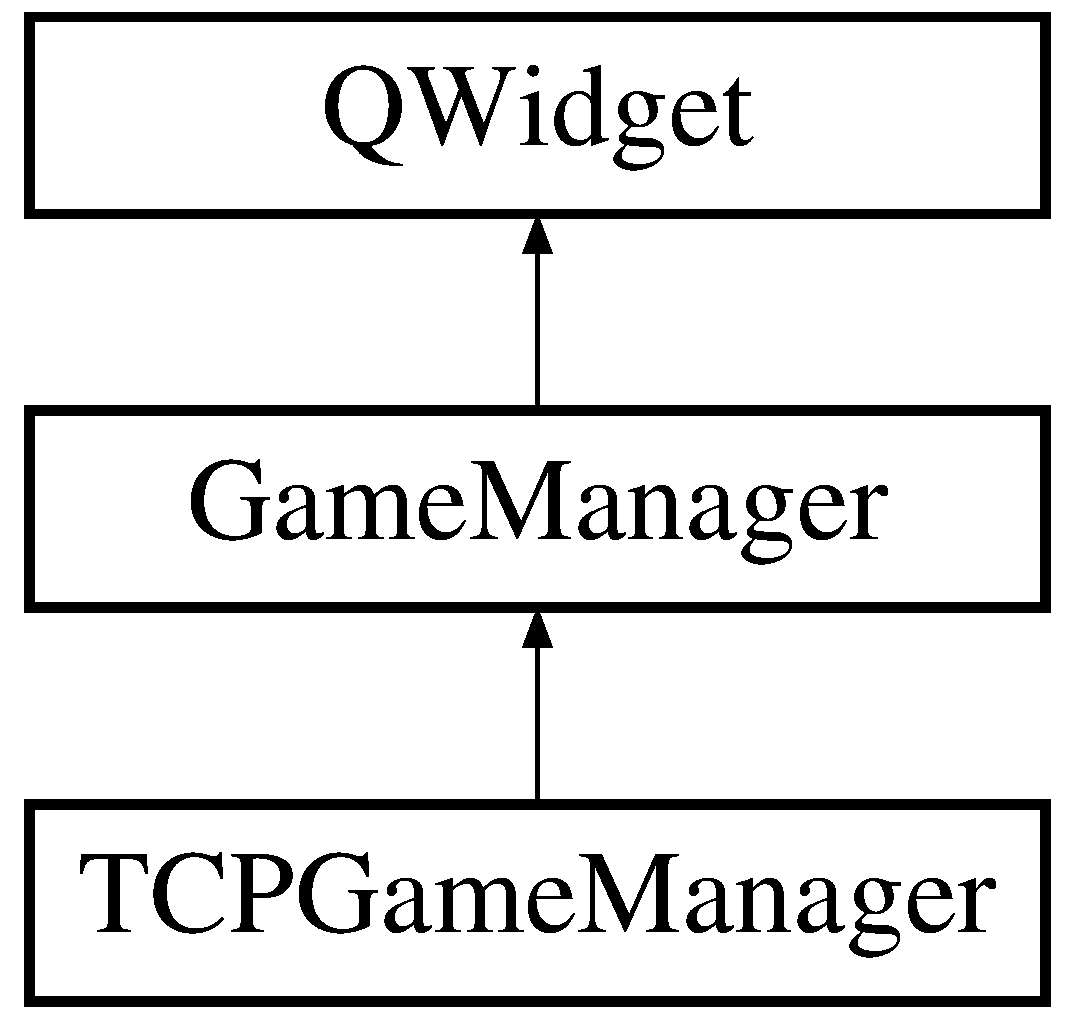
\includegraphics[height=3.000000cm]{class_t_c_p_game_manager}
\end{center}
\end{figure}
\subsection*{Public Slots}
\begin{DoxyCompactItemize}
\item 
\hypertarget{class_t_c_p_game_manager_a616b05b986023096f7475e32c70a059d}{void {\bfseries client\-Connected} ()}\label{class_t_c_p_game_manager_a616b05b986023096f7475e32c70a059d}

\item 
\hypertarget{class_t_c_p_game_manager_a65421be056b0c53a6deed1bd405ffc6b}{void {\bfseries connection\-Established} ()}\label{class_t_c_p_game_manager_a65421be056b0c53a6deed1bd405ffc6b}

\item 
\hypertarget{class_t_c_p_game_manager_a6412d2d4a43e5ff353d410e810f60675}{void {\bfseries received\-Data} (const Q\-String \&data)}\label{class_t_c_p_game_manager_a6412d2d4a43e5ff353d410e810f60675}

\end{DoxyCompactItemize}
\subsection*{Signals}
\begin{DoxyCompactItemize}
\item 
\hypertarget{class_t_c_p_game_manager_ab3a7b1cacfd6ca1704d683f5bc794d98}{void \hyperlink{class_t_c_p_game_manager_ab3a7b1cacfd6ca1704d683f5bc794d98}{chat\-Message\-Received} (Q\-String message)}\label{class_t_c_p_game_manager_ab3a7b1cacfd6ca1704d683f5bc794d98}

\begin{DoxyCompactList}\small\item\em emitted when a new chat message has been received \end{DoxyCompactList}\end{DoxyCompactItemize}
\subsection*{Public Member Functions}
\begin{DoxyCompactItemize}
\item 
\hypertarget{class_t_c_p_game_manager_a0a83c4efd02332883aaa7935b480ec2c}{{\bfseries T\-C\-P\-Game\-Manager} (Q\-Widget $\ast$parent)}\label{class_t_c_p_game_manager_a0a83c4efd02332883aaa7935b480ec2c}

\item 
\hypertarget{class_t_c_p_game_manager_a7d4415253458e80a05314f91a0879fd0}{void \hyperlink{class_t_c_p_game_manager_a7d4415253458e80a05314f91a0879fd0}{start\-Game} (\hyperlink{struct_settings}{Settings} settings)}\label{class_t_c_p_game_manager_a7d4415253458e80a05314f91a0879fd0}

\begin{DoxyCompactList}\small\item\em instanciates renderer and gameboard \end{DoxyCompactList}\item 
\hypertarget{class_t_c_p_game_manager_a518a1a16b52b9ede6474749f59f203b1}{void {\bfseries send\-Message} (Q\-String string)}\label{class_t_c_p_game_manager_a518a1a16b52b9ede6474749f59f203b1}

\end{DoxyCompactItemize}
\subsection*{Protected Member Functions}
\begin{DoxyCompactItemize}
\item 
\hypertarget{class_t_c_p_game_manager_af76ec973ba1c3e7f58ac979fffccb85f}{void {\bfseries mouse\-Press\-Event} (Q\-Mouse\-Event $\ast$event)}\label{class_t_c_p_game_manager_af76ec973ba1c3e7f58ac979fffccb85f}

\end{DoxyCompactItemize}
\subsection*{Protected Attributes}
\begin{DoxyCompactItemize}
\item 
\hypertarget{class_t_c_p_game_manager_aabea99b1b4ed457eff4a5f0db194644b}{bool {\bfseries m\-\_\-\-Network\-Initialized}}\label{class_t_c_p_game_manager_aabea99b1b4ed457eff4a5f0db194644b}

\item 
\hypertarget{class_t_c_p_game_manager_a762b0b3ae60c0076165843b78d011927}{bool {\bfseries m\-\_\-\-Server\-Turn}}\label{class_t_c_p_game_manager_a762b0b3ae60c0076165843b78d011927}

\item 
\hypertarget{class_t_c_p_game_manager_ad973154be37079b7510d4ca3d66d47fb}{bool {\bfseries m\-\_\-\-Sent\-But\-Not\-Received}}\label{class_t_c_p_game_manager_ad973154be37079b7510d4ca3d66d47fb}

\item 
\hypertarget{class_t_c_p_game_manager_a15acfb9058bd60dbaad4a9561f643da3}{std\-::shared\-\_\-ptr\\*
$<$ \hyperlink{class_server_search_listener}{Server\-Search\-Listener} $>$ {\bfseries m\-\_\-p\-Server\-Search\-Listener}}\label{class_t_c_p_game_manager_a15acfb9058bd60dbaad4a9561f643da3}

\end{DoxyCompactItemize}


\subsection{Detailed Description}
Gamemanager that handles Network game related tasks. 

Definition at line 11 of file tcpgamemanager.\-h.



The documentation for this class was generated from the following files\-:\begin{DoxyCompactItemize}
\item 
tcpgamemanager.\-h\item 
tcpgamemanager.\-cpp\end{DoxyCompactItemize}

%--- End generated contents ---

% Index
\newpage
\phantomsection
\addcontentsline{toc}{chapter}{Index}
\printindex

\end{document}
